% !TEX program = lualatex
\documentclass[11pt,a4paper]{article}

\usepackage{fontspec}
\usepackage{polyglossia}
\usepackage{csquotes}
\usepackage{amsmath,amssymb}
\usepackage{booktabs}
\usepackage{tabularx}
\usepackage{enumitem}
\usepackage{hyperref}
\usepackage{xcolor}
\usepackage{listings}
\usepackage{tikz}
\usepackage{graphicx}
\usepackage{geometry}
\usepackage{fancyhdr}
\usepackage{titlesec}

\geometry{margin=2.4cm}
\setdefaultlanguage{russian}
\setotherlanguage{english}
\setmainfont{Charis SIL}[Ligatures=TeX]
\setsansfont{DejaVu Sans}[Ligatures=TeX]
% Фирменные шрифты Isabelle (contrib/isabelle_fonts) для кода и утверждений
\setmonofont{IsabelleDejaVuSansMono}[
  Path=fonts/,
  Extension=.ttf,
  UprightFont=*,
  BoldFont=*-Bold,
  ItalicFont=*-Oblique,
  BoldItalicFont=*-BoldOblique,
  Scale=0.95
]
\newfontfamily\cyrillicfont{Charis SIL}[Ligatures=TeX]
\newfontfamily\cyrillicfontsf{DejaVu Sans}[Ligatures=TeX]
\newfontfamily\cyrillicfonttt{IsabelleDejaVuSansMono}[
  Path=fonts/,
  Extension=.ttf,
  UprightFont=*,
  BoldFont=*-Bold,
  ItalicFont=*-Oblique,
  BoldItalicFont=*-BoldOblique,
  Scale=0.95
]
% Стиль Isabelle-документа (\isabellestyle{it}): имена лемм/теорем курсивом
\newfontfamily\isabelleit{IsabelleDejaVuSerif}[
  Path=fonts/,
  Extension=.ttf,
  UprightFont=*-Italic,
  BoldFont=*-BoldItalic,
  ItalicFont=*-Italic,
  BoldItalicFont=*-BoldItalic,
  Scale=0.97,
  Ligatures=TeX
]
\newcommand{\isabel}[1]{{\isabelleit #1}}
\newcommand{\lemmaname}[1]{\isabel{#1}}

\usetikzlibrary{arrows.meta,positioning,fit,calc,shapes.multipart}

\hypersetup{
  colorlinks=true,
  linkcolor=black!70,
  urlcolor=blue!50!black,
  pdftitle={Микроверификация capability-модели в стиле Zircon в Isabelle/HOL},
  pdfauthor={redbeardster}
}

\definecolor{codebg}{RGB}{248,248,245}
\definecolor{codekw}{RGB}{120,40,80}
\definecolor{codestr}{RGB}{40,90,40}
\definecolor{codecom}{RGB}{100,100,100}
\definecolor{accent}{RGB}{30,90,120}

\lstdefinelanguage{Isabelle}{
  morekeywords={definition,lemma,theorem,assumes,shows,where,using,by,auto,
    simp,blast,case,of,if,then,else,in,let,Some,None,and,theory,imports,
    begin,end,record,datatype,type_synonym,locale,interpretation,fixes},
  sensitive=true,
  morecomment=[l]{\%},
  morecomment=[n]{(*}{*)},
  morestring=[b]"
}

\lstset{
  language=Isabelle,
  basicstyle=\ttfamily\small,
  keywordstyle=\color{codekw}\bfseries,
  commentstyle=\color{codecom}\itshape,
  stringstyle=\color{codestr},
  backgroundcolor=\color{codebg},
  frame=single,
  rulecolor=\color{black!20},
  breaklines=true,
  columns=fullflexible,
  keepspaces=true,
  showstringspaces=false,
  aboveskip=0.8em,
  belowskip=0.8em,
  xleftmargin=0.4em,
  xrightmargin=0.4em,
  literate=
    {⇒}{{$\Rightarrow$}}1
    {⟹}{{$\Longrightarrow$}}1
    {→}{{$\rightarrow$}}1
    {↦}{{$\mapsto$}}1
    {∩}{{$\cap$}}1
    {∈}{{$\in$}}1
    {∉}{{$\notin$}}1
    {∃}{{$\exists$}}1
    {∄}{{$\nexists$}}1
    {¬}{{$\neg$}}1
    {∧}{{$\land$}}1
    {≤}{{$\le$}}1
    {⊑}{{$\sqsubseteq$}}1
    {⟷}{{$\longleftrightarrow$}}1
}

\titleformat{\section}{\Large\bfseries\color{accent}}{\thesection.}{0.6em}{}
\titleformat{\subsection}{\large\bfseries}{\thesubsection.}{0.5em}{}

% Баннер инженерной врезки
\definecolor{insetborder}{RGB}{30,90,120}
\definecolor{insetbg}{RGB}{245,248,250}
\newcommand{\enginsetbanner}[1]{%
  \par\medskip\noindent
  \begin{tikzpicture}
    \node[
      draw=insetborder,
      line width=0.9pt,
      fill=insetbg,
      inner sep=0.85em,
      text width=\dimexpr\linewidth-1.7em\relax,
      align=justify,
      rounded corners=1.5pt
    ]
    {\textbf{\color{insetborder}Инженерная врезка.}~
     #1};
  \end{tikzpicture}%
  \par\medskip
}

\pagestyle{fancy}
\fancyhf{}
\fancyhead[L]{\small Учебная \textenglish{capability}-модель в стиле Zircon}
\fancyhead[R]{\small Isabelle/HOL}
\fancyfoot[C]{\thepage}
\renewcommand{\headrulewidth}{0.3pt}

\begin{document}

\begin{center}
	{\LARGE\bfseries Учебная модель \textenglish{capability}-делегирования}\\[0.35em]
	{\Large в стиле Zircon (Fuchsia~OS) средствами Isabelle/HOL}\\[1em]
	{\large redbeardster@gmail.com}\\[0.3em]
	{\normalsize 2026}
\end{center}

\vspace{0.6em}

\begin{abstract}
	\noindent
	В работе построена \emph{учебная} формальная модель фрагмента
	\textenglish{capability}-механизма в стиле микроядра Zircon
	(Fuchsia~OS) в Isabelle/HOL. Доступ к объектам ядра в Zircon идёт
	через дескрипторы с масками прав; ключевой вопрос делегирования~---
	не получает~ли получатель при передаче прав сверх источника. Мы
	доказываем отсутствие такой эскалации для композиции
	\lemmaname{transfer\_via\_channel} (успешный
	\texttt{write}/\texttt{read} при \emph{пустой} очереди получателя)
	на всех состояниях, достижимых из корректного старта
	(\texttt{state\_wf}). Той~же моделью показана граница гарантии:
	гипотетический привилегированный poke в store VMO (в духе обхода
	мимо шлюза прав, а не полная модель
	\texttt{ZX\_RSRC\_KIND\_MMIO}) ломает изоляцию содержимого, хотя
	проверки \textenglish{capability} на syscall-пути остаются на месте.
	Модель намеренно упрощена и не претендует на верификацию
	промышленного Zircon.
\end{abstract}

\paragraph{Соглашения о терминологии.}
В тексте мы сохраняем английские термины, устоявшиеся в
security-литературе, но при первом употреблении даём русский перевод и
краткое пояснение в скобках. Ключевые термины:
\emph{capability} (полномочие)~--- объект-носитель права доступа к
ресурсу ядра;
\emph{handle} (дескриптор)~--- слот в таблице процесса, ссылающийся на
\textenglish{capability};
\emph{refinement} (уточнение)~--- доказательство того, что
низкоуровневая реализация является допустимым поведением
высокоуровневой спецификации;
\emph{attenuation} (ослабление, урезание прав)~--- свойство передачи не
давать получателю больше прав, чем было у источника;
\emph{capability-маска} (rights mask)~--- множество атомарных прав у
конкретного \textenglish{capability};
\emph{witness} (свидетель)~--- конкретный объект или сценарий,
подтверждающий выполнимость утверждения;
\emph{negative witness} (негативный свидетель)~--- контрпример,
опровергающий утверждение;
\emph{syscall} (системный вызов)~--- вызов ядра из пользовательского
процесса;
\emph{VMO} (Virtual Memory Object, виртуальный объект памяти)~---
разделяемый объект памяти ядра Zircon;
\emph{MMIO} (Memory-Mapped I/O)~--- отображённый в адресное пространство
доступ к регистрам устройств;
\emph{сессия} (Isabelle session)~--- именованный набор теорий, который
Isabelle проверяет одной командой сборки (у нас
\texttt{isabelle build -d . Zircon} и шесть теорий
\texttt{Portable\_Capability}, \texttt{Zircon}, \texttt{Zircon\_Lattice},
\texttt{Zircon\_Traces}, \texttt{Zircon\_MMIO}, \texttt{Zircon\_Code});
это единица сборки proof assistant'а, а не «сеанс работы за компьютером»
и не HTTP-сессия.

\paragraph{Граница модели.}
Наша модель намеренно упрощена и не претендует на верификацию промышленного ядра Zircon
в объёме проектов класса seL4. Это учебная формализация фрагмента логики прав, а не полный Zircon API.
Наш \texttt{zx\_channel\_write}~--- прообраз
\texttt{zx\_channel\_write\_etc} с одной записью
\texttt{zx\_handle\_disposition\_t}
(\texttt{ZX\_HANDLE\_OP\_MOVE}, \texttt{rights = req}): там
\texttt{rights}~--- «desired final rights (not a mask)», и запрос сверх
прав источника даёт \texttt{ZX\_ERR\_INVALID\_ARGS}~--- у нас проверка
$\mathit{req}\subseteq h\_rights$. Это \emph{прообраз} одного
\texttt{MOVE}, а не тождество: у \texttt{write\_etc} при допустимом
запросе получатель берёт ровно \texttt{req} («desired final rights»),
у нас затем \lemmaname{reduce\_rights\_wf} может дописать
\texttt{READ} по учебной зависимости (см.\ ниже); нет байт сообщения,
нет массива handles и нет \texttt{DUPLICATE} в disposition.
При ошибке у нас \texttt{None} не меняет состояние. У обычного
\texttt{zx\_channel\_write} handles сбрасываются и при отказе; у
\texttt{write\_etc} с \texttt{ZX\_HANDLE\_OP\_MOVE} источник
\emph{тоже} закрывается (эквивалент \texttt{zx\_handle\_replace} затем
write, «always closed»). Учебный freeze-on-\texttt{None}~--- не
семантика ядра.
\lemmaname{create\_channel\_pair} склеивает \texttt{zx\_channel\_create}
(оба конца~--- создателю) с доставкой второго конца в другой процесс;
композиция \lemmaname{transfer\_via\_channel} дополнительно требует
пустую очередь получателя~--- в Zircon write в непустую очередь
допустим. MMIO-обход в~§9~--- гипотетический poke в
\texttt{vmo\_store} по \texttt{obj\_id} (тип \texttt{Hardware} его не
ограничивает), а не путь через \texttt{ZX\_RSRC\_KIND\_MMIO}/BTI.
Зависимость
\texttt{WRITE}$\Rightarrow$\texttt{READ} (и \texttt{EXECUTE}$\Rightarrow$\texttt{READ})
учебная: в Zircon эти биты независимы, ядро \texttt{READ} само не
дописывает. Замыкание копирует \texttt{READ} у уже корректного
источника, а не чеканит новое право (подробнее~--- §8.5). Два конца
канала с \texttt{channel\_peer}, проверка \texttt{DUPLICATE} и симметрия
пиров как инвариант трассы в модели есть. Полный перечень отличий~--- по
ходу §3--§5 и в теориях.

\section{Введение}

Контроль доступа к объектам ядра относится к числу механизмов, ошибки в
которых непосредственно ведут к уязвимостям класса Local Privilege
Escalation. Традиционные средства обеспечения качества~--- модульное
тестирование, обзор кода, фаззинг~--- эффективно выявляют конкретные
дефекты реализации, однако не устанавливают общезначимых свойств вида
«для всякого состояния, достижимого из корректного старта, передача
\textenglish{capability} не увеличивает множество прав». Формальная верификация восполняет этот пробел, но часто
ассоциируется исключительно с крупномасштабными проектами (например,
seL4~\cite{sel4,sel4overview}), требующими многолетних усилий
специализированных групп.

\paragraph{Что мы называем эскалацией.}
Прежде чем переходить к формализации, зафиксируем рабочее определение.
\emph{Эскалацией прав} мы называем ситуацию, когда после операции у
получателя появляется право, которого у источника не было:
$h\_rights(\text{получателя}) \not\subseteq h\_rights(\text{источника})$.
Требование «отсутствия эскалации» означает: такого состояния не существует
\emph{ни при каком} сценарии из корректного начального состояния
(\texttt{state\_wf} и трасса \texttt{reachable})~--- то
есть это утверждение обо всех \emph{достижимых} состояниях модели, а не о
конкретном тесте и не о произвольной HOL-записи с «битой» маской.
Именно это свойство доказывается ниже для передачи
\textenglish{capability} через канал~--- в форме композиции
\lemmaname{transfer\_via\_channel}, которая дополнительно требует
пустую очередь получателя (см.\ границу модели); у одиночного
\lemmaname{zx\_channel\_write} пустота не нужна.

Цель настоящей статьи~--- показать, что \emph{базовые} архитектурные
инварианты \textenglish{capability}-модели допускают компактную формализацию и
автоматизированную проверку в Isabelle/HOL без построения полной
семантики ядра. На учебной модели в стиле Zircon доказаны, в частности:
\begin{itemize}[leftmargin=1.4em]
	\item \lemmaname{channel\_transfer\_no\_escalation}~--- нет эскалации при
	      передаче через канал;
	\item \lemmaname{channel\_write\_requires\_transfer}~--- без
	      \texttt{TRANSFER} отправка невозможна;
	\item \lemmaname{channel\_write\_moves\_sender\_handle}~--- move у
	      отправителя;
	\item \lemmaname{vmo\_write\_denied\_without\_write\_right}~--- запись в
	      VMO без \texttt{WRITE} отвергается;
	\item \lemmaname{mmio\_leak\_witness\_true}~--- привилегированный MMIO-обход
	      ломает системную изоляцию store при живом capability-шлюзе;
	\item \lemmaname{zx\_handle\_duplicate\_no\_escalation}~--- то~же
	      сокращение прав (meet + замыкание) при дублировании handle.
\end{itemize}
Предполагается знакомство читателя с функциональным программированием;
специальная подготовка в области математической логики не требуется.

\paragraph{Отношение к seL4.}
Проект seL4~\cite{sel4,sel4overview} даёт полный \emph{refinement}
(уточнение~--- пошаговое доказательство того, что каждая
низкоуровневая реализация является допустимым поведением
высокоуровневой спецификации) от абстрактной спецификации до
бинарника. Настоящая работа~--- иного масштаба и цели: компактное
доказательство того~же \emph{типа} свойства (\emph{no rights
	escalation}~--- отсутствие эскалации прав, то есть получатель не
приобретает прав, которых не было у источника) для узкого фрагмента
системных вызовов и явный контрпример к системным обещаниям при обходе
через MMIO. Помимо самого результата~--- полной верификации ядра~---
seL4 даёт переносимую методологию: \emph{refinement}-стек из
нескольких уровней, архитектуру под \emph{tractability} (податливость
формальному доказательству: ядро спроектировано так, чтобы его
инварианты вообще допускали машинную проверку) и доказательство
\emph{access-control enforcement} (принудительное соблюдение контроля
доступа: политика не только формулируется, но и гарантированно
применяется на каждом переходе). Наш фрагмент не воспроизводит эту
методологию целиком; он выделяет один её слой~--- монотонное
\emph{attenuation} (ослабление, урезание прав при передаче:
получатель не может приобрести прав больше, чем было у источника)
\textenglish{capability}-масок~--- и показывает, что даже этот слой
даёт содержательные машинно проверяемые гарантии без построения
полной семантики ядра. Разница не в «меньшей строгости», а в
назначении: seL4~--- для сертификации ядра; наша модель~--- для
\emph{ранней} проверки архитектурных решений и обучения языку
формальных инвариантов делегирования.

Прежде чем углубляться в формализацию, зафиксируем
\emph{проверяемый} контекст по документации Fuchsia: зачем инварианты
\textenglish{capability}-модели Zircon интересны инженеру и где типичная
точка напряжения~--- MMIO и слои совместимости.

\section{Контекст: актуальность формальной проверки \textenglish{capability}-модели}

\subsection{Индустриальный фон}

Fuchsia~--- операционная система с микроядром Zircon; доступ к объектам
ядра строится на \textenglish{capability}-дисциплине: процесс работает с
ресурсом только через handle с явной маской
прав~\cite{zircon_handles,zircon_rights}. Эта дисциплина заявлена как
основа безопасности и модульности системы. Вопрос настоящей работы не
в~том, «хороша~ли идея в принципе», а в~том, можно~ли
\emph{машинно проверить} узкий, но критичный инвариант делегирования:
передача не увеличивает множество прав,~--- без полной семантики ядра.

\subsection{Архитектурный конфликт и место формальной модели}

Типичная точка напряжения~--- драйверы периферии, обращающиеся к
регистрам через memory-mapped~I/O (MMIO). В Linux такой драйвер часто
живёт в привилегированном режиме. В Fuchsia произвольная запись
userspace в физическую память \emph{не} свободна: доступ к MMIO-диапазонам
выдаётся через ресурсы вида \texttt{ZX\_RSRC\_KIND\_MMIO} и связанные
механизмы~\cite{zircon_mmio}. Параллельно развивается Starnix~--- слой,
эмулирующий Linux-подобные системные вызовы поверх
Zircon~\cite{zircon_starnix}; маршрутизация capabilities к контейнеру и
к \texttt{starnix\_kernel} там тоже часть дисциплины прав.

Тем не менее исключение вида «открыть чрезмерно широкий MMIO» без узкой
маски разрушает смысл \textenglish{capability}: процесс с широким доступом к
железу снова может записать «что угодно куда угодно», и дефект драйвера
превращается в угрозу целостности ядра~--- ровно то, от чего микроядерная
модель должна защищать. Переписывание драйверов и интерфейсов под
нативную модель Zircon дорого (IPC, FIDL, границы устройств); без
формального языка инвариантов доверие к делегированию прав остаётся
декларативным.

Модульные тесты и фаззинг находят конкретные дефекты и не устанавливают
свойство вида «ни при каком допустимом состоянии передача handle не
увеличивает множество прав». Специалисту по безопасности нужен язык
спецификации и способ \emph{опровергнуть} небезопасную архитектуру ещё
до внедрения в код.

Настоящая заметка~--- методический мост между документацией
Zircon~\cite{zircon_handles,zircon_rights} и машинно проверяемым
фрагментом логики прав: handles/каналы/VMO, отсутствие эскалации, шлюз
\texttt{TRANSFER}, целостность записи, решётка, экстракция в OCaml.
Цепочка~--- «архитектура $\to$ доказательство $\to$ исполняемый
артефакт»; модель учебная и не покрывает полный syscall surface.

\subsection{Ценность для специалистов по безопасности}

Для аудитории, работающей в области безопасности приложений и
операционных систем (\emph{application / OS security}), эта работа
полезна не как замена полного аудита Zircon, а как
\emph{инструментальный образец}.
\begin{description}[style=nextline,leftmargin=1.2em]
	\item[Язык спецификации]
	      Требования к \textenglish{capability}-фрагменту формулируются на языке, который
	      понимает доказатель; неоднозначность проектной документации
	      снижается.
	\item[Раннее обнаружение дефектов]
	      Если инвариант не доказывается, архитектура отвергается на этапе
	      модели, а не после инцидента (пример с пропущенным
	      \texttt{TRANSFER}~--- в~§7.1).
	\item[Перепроверяемые гарантии]
	      Результат~--- не только экспертное мнение, а артефакт, который можно
	      пересобрать (\texttt{isabelle build}, \texttt{test\_code}, OCaml-прогон).
	\item[Обучение и практики]
	      Компактный пример показывает минимальный набор свойств, которые
	      имеет смысл требовать от \textenglish{capability}-IPC до масштабирования на полное
	      ядро.
\end{description}
Ограничение остаётся явным: модель учебная и не покрывает драйверы,
Starnix и полный syscall surface; MMIO входит лишь как
\emph{контрпример обхода} (§9), а не как полная модель железа.
Тем не менее даже такой фрагмент
даёт содержательную информацию: инвариант "нет эскалации" может быть
доказан \emph{локально}, без моделирования всей ОС. Ценность для
security-инженера~--- в достижимости формального метода для критичного
узла и в шаблоне расширения к тем местам, где безопасность сталкивается
с совместимостью.

\section{Абстракция: от полного ядра к модели прав}

Полная семантика Zircon включает процессы, обширный интерфейс системных
вызовов и средства синхронизации. Для анализа логики прав достаточно
выделить минимальный набор сущностей и операций.

\subsection{Онтология}

\begin{enumerate}[leftmargin=1.6em,label=\arabic*.,ref=\arabic*]
	\item \textbf{Идентификаторы.}
	      \texttt{process\_id}, \texttt{handle\_id}, \texttt{obj\_id}
	      моделируются типом \texttt{nat}. Выбор отражает интерес к логическим
	      свойствам, а не к битовому представлению 32-разрядных дескрипторов.
	      Очереди каналов индексируются \texttt{obj\_id} объекта типа
	      \texttt{Channel}.
	\item \textbf{Объект ядра.}
	      Пара $\langle\texttt{тип},\,\texttt{id}\rangle$, где тип принадлежит
	      конечному перечислению
	      (\texttt{Process}, \texttt{Thread}, \texttt{Channel}, \texttt{VMO},
	      а также \texttt{Hardware} и \texttt{Other\_Obj}~--- задел
	      расширяемости; poke в~§9 бьёт в \texttt{vmo\_store} по
	      \texttt{obj\_id} и тип объекта не проверяет).
	\item \textbf{Handle} (дескриптор).
	      Ссылка на объект вместе с множеством атомарных прав
	      (\textenglish{capability-маска}, rights mask): \texttt{record} с
	      полями \texttt{h\_obj}, \texttt{h\_rights}. Именно слот
	      \texttt{handle} в таблице процесса несёт право доступа; передача
	      \texttt{handle} и есть передача полномочия.
	\item \textbf{Capability} (полномочие).
	      В модели это \emph{тот~же тип}:
	      \texttt{type\_synonym capability = handle}. Имя
	      \texttt{capability} подчёркивает роль «в полёте» по каналу
	      (без локального \texttt{handle\_id} получателя~--- он появится при
	      \texttt{read}); проекция \texttt{h\_rights} поэтому законна и для
	      элементов \texttt{capability list}.
	      Отметим: склейка \texttt{capability} и \texttt{handle} в один
	      тип~--- учебное упрощение представления. В реальном Fuchsia
	      права тоже ассоциированы с \emph{handle}
	      (\emph{«Rights are associated with handles»}~\cite{zircon_rights}),
	      а не с записью объекта в таблице ядра; несколько дескрипторов
	      на один объект могут нести разные маски. Наша склейка удобна
	      для модели, но не воспроизводит полное разделение «слот в
	      таблице процесса» / «объект ядра».
	\item \textbf{Состояние системы} включает:
	      \begin{enumerate}[leftmargin=1.4em,label=\alph*)]
		      \item \texttt{proc\_tables}~--- таблицы дескрипторов процессов;
		      \item \texttt{channels}~--- очереди capabilities по концам
		            каналов (\texttt{obj\_id $\rightharpoonup$ capability list});
		      \item \texttt{channel\_peer}~--- связь конца с противоположным
		            (\texttt{obj\_id $\rightharpoonup$ obj\_id});
		      \item \texttt{vmo\_store}~--- абстрактное содержимое VMO
		            (\texttt{obj\_id $\rightharpoonup$ nat});
		      \item счётчики для выделения свежих идентификаторов
		            (\texttt{next\_hids}, \texttt{next\_obj\_id}).
		            Свежие \texttt{handle\_id} выделяет
		            \texttt{alloc\_hid~pid~s}, возвращая пару
		            (новый~id,~обновлённое состояние со сдвинутым счётчиком);
		            нумерация с~1, поскольку в Zircon
		            \texttt{0 = ZX\_HANDLE\_INVALID}.
	      \end{enumerate}
\end{enumerate}
\paragraph{Частичная функция.}
Запись $\alpha \rightharpoonup \beta$~--- стандартное для Isabelle
обозначение \emph{частичной функции} из $\alpha$ в $\beta$: она либо
возвращает \texttt{Some}~$y$, либо \texttt{None}, если значения нет.
В терминах теории типов это $\alpha \Rightarrow \beta~\texttt{option}$.
Такая форма удобна, когда таблица «разрежена»: у не всех
\texttt{handle\_id} есть дескриптор. Именно поэтому
\lemmaname{lookup\_handle} и \lemmaname{get\_table} возвращают
\texttt{option}, а не отдельный \texttt{bool}-признак вместе со
значением: отсутствие дескриптора и «дескриптор с пустой маской»~---
разные состояния.

\paragraph{Короткое пояснение к флагам.}
Перечисленные в модели права покрывают минимум, необходимый для сценариев
статьи. \texttt{ZX\_RIGHT\_READ} и \texttt{ZX\_RIGHT\_WRITE} разрешают
соответственно читать и модифицировать объект.
\texttt{ZX\_RIGHT\_EXECUTE} разрешает исполнение кода из объекта
(актуально для VMO). \texttt{ZX\_RIGHT\_MAP} разрешает отображать
объект в адресное пространство процесса.
\texttt{ZX\_RIGHT\_TRANSFER} разрешает передавать handle другим
процессам через канал~--- именно это право проверяет
\lemmaname{zx\_channel\_write}. \texttt{ZX\_RIGHT\_DUPLICATE}
обязателен для \lemmaname{zx\_handle\_duplicate}.
\texttt{ZX\_RIGHT\_SIGNAL} в текущих сценариях не задействован и
приведён для полноты перечня относительно настоящего Zircon
(где есть также WAIT, DESTROY, property/policy rights).

Поле \texttt{proc\_tables}~--- это частичная функция, принимающая на
вход пару (идентификатор процесса, идентификатор дескриптора) и
возвращающая полномочие~--- пару «объект ядра + маска прав». Если для
данной пары слот не заполнен, функция возвращает «пусто»
(\texttt{None}); при этом отсутствие дескриптора и «дескриптор с
пустой маской»~--- два разных состояния, и мы их не смешиваем.

Каждый системный вызов~--- это атомарная транзакция над
\texttt{system\_state}: таблицы дескрипторов (\texttt{proc\_tables})
часто в центре внимания, но тот~же шаг может менять и другие поля
(например, очереди \texttt{channels}). Либо состояние целиком
переходит в новое (\texttt{Some~$s'$}), либо остаётся неизменным
(\texttt{None}). Промежуточного, частично обновлённого состояния не
бывает. Модель последовательная: переходы~---
атомарные шаги. Это не только упрощение доказательства, но и
содержательное допущение: локальные инварианты \textenglish{capability}
доказуемы именно потому, что шаг неделим. Конкурентность~---
одновременное обращение нескольких потоков к таблицам дескрипторов~---
сознательно вынесена за рамки модели.

Отдельная оговорка о времени жизни объектов. В промышленном Zircon
на один объект ядра может ссылаться несколько дескрипторов~--- в
одной таблице или в разных; в модели это тоже есть
(\lemmaname{zx\_handle\_duplicate} создаёт второй handle на тот~же
объект). Чего в модели нет~--- подсчёта ссылок (\emph{refcounting}):
у объекта Zircon есть счётчик, и объект уничтожается, когда закрыт
последний handle. У нас \lemmaname{zx\_handle\_close} удаляет слот, но
объект и его запись в \texttt{vmo\_store} остаются. Добавление подсчёта
ссылок~--- это расширение инварианта корректности состояния
(\texttt{state\_wf}, определён ниже), а не переопределение самих
операций.

Наконец, политика порождения новых прав (\emph{minting}) при создании
объектов (\texttt{create\_vmo}, \texttt{create\_channel\_pair}) тоже
остаётся вне модели: начальные маски задаются снаружи и не выводятся
из прав «родителя». Модель доказывает ослабление прав при передаче и
при дублировании дескриптора (\lemmaname{zx\_handle\_duplicate}), а не
корректность того, \emph{кто} вправе породить объект с данной маской.

\paragraph{Канал как \textenglish{capability}-объект.}
Очередь канала адресуется через handle на
endpoint~--- ту же дисциплину, что и для VMO. Ключ в
\texttt{channels}~--- \texttt{obj\_id} объекта типа \texttt{Channel};
писать и читать очередь можно только после \texttt{lookup\_handle} с
проверкой \texttt{ZX\_RIGHT\_WRITE} / \texttt{ZX\_RIGHT\_READ}:
\begin{lstlisting}
channels :: "obj_id ⇀ capability list"

zx_channel_write ::
  "process_id ⇒ handle_id ⇒ handle_id ⇒ rights ⇒
   system_state ⇒ system_state option"
  (* pid, channel endpoint, payload, requested rights *)

vmo_write ::
  "process_id ⇒ handle_id ⇒ nat ⇒
   system_state ⇒ system_state option"
\end{lstlisting}
Пара эндпоинтов создаётся \lemmaname{create\_channel\_pair}: два объекта
\texttt{Channel} со своими очередями и взаимной связью
\texttt{channel\_peer}. Запись кладёт сообщение в очередь
\emph{пира}, чтение забирает из \emph{своей}~--- как в Zircon.
Оговорка: настоящий \texttt{zx\_channel\_create} возвращает \emph{оба}
конца создателю, с одинаковыми правами по умолчанию
(\texttt{TRANSFER|READ|WRITE|WAIT|INSPECT|SIGNAL|SIGNAL\_PEER}); второй
конец попадает в другой процесс через bootstrap-handle при
\texttt{zx\_process\_start} или по уже существующему каналу. Наша операция
склеивает «создать + доставить» в один шаг и позволяет задать маски
концов независимо~--- это учебное упрощение, а не отдельный syscall.
Рис.~\ref{fig:channel-handles} показывает единый путь доступа через handle.

\begin{figure}[ht]
	\centering
	\begin{tikzpicture}[
			font=\footnotesize,
			>=Latex,
			box/.style={draw=accent!65, rounded corners=2pt, align=center,
					inner sep=4pt, fill=accent!4,
					font=\sffamily\footnotesize},
			lab/.style={font=\sffamily\scriptsize\bfseries, text=accent!90},
			arr/.style={->, thick, accent!75}
		]
		\node[lab] (t) at (3.6,2.55) {Микромодель = дисциплина Zircon};
		\node[box] (p) at (3.6,1.85) {Процесс};
		\node[box] (hc) at (1.2,0.85) {handle на Channel\\[0.5pt]
			\texttt{\scriptsize WRITE/READ}};
		\node[box] (hv) at (6.0,0.85) {handle на VMO\\[0.5pt]
			\texttt{\scriptsize TRANSFER/WRITE}};
		\node[box] (q) at (1.2,-0.25) {\texttt{\scriptsize channels oid}\\[0.5pt]
			очередь payload};
		\node[box] (v) at (6.0,-0.25) {\texttt{\scriptsize vmo\_write}\\[0.5pt]
			через \texttt{\scriptsize lookup\_handle}};
		\draw[arr] (p) -- (hc);
		\draw[arr] (p) -- (hv);
		\draw[arr] (hc) -- (q);
		\draw[arr] (hv) -- (v);
	\end{tikzpicture}
	\caption{Единая \textenglish{capability}-адресация: и канал, и VMO доступны только через
		handle в \texttt{proc\_tables}.}
	\label{fig:channel-handles}
\end{figure}

Дополнительно \lemmaname{zx\_channel\_write} реализует \emph{move}: после
успеха \texttt{lookup\_handle pid pay\_hid s' = None}
(\lemmaname{channel\_write\_moves\_sender\_handle}). Инварианты
no-escalation относятся к маске прав у payload. Отношение к
промышленному Zircon: обычный \texttt{zx\_channel\_write} маску не
принимает, но \texttt{zx\_channel\_write\_etc} принимает~--- для
каждого handle задаётся \texttt{zx\_handle\_disposition\_t} с
операцией (\texttt{MOVE}/\texttt{DUPLICATE}) и желаемыми итоговыми
правами; запрос сверх прав источника~---
\texttt{ZX\_ERR\_INVALID\_ARGS}, попытка отправить канал в самого
себя~--- \texttt{ZX\_ERR\_NOT\_SUPPORTED}. Наша операция~--- \emph{прообраз} \texttt{write\_etc} с одной
\texttt{MOVE}-записью: проверка
$\mathit{req}\subseteq h\_rights$, затем
\lemmaname{reduce\_rights\_wf} (учебное замыкание зависимостей: итог
может быть шире \texttt{req}, если замыкание дописывает
\texttt{READ}), плюс
\texttt{WRITE} на канал и \texttt{TRANSFER} на
payload~\cite{zircon_rights,zircon_handles}. Как и в \texttt{write\_etc},
\texttt{TRANSFER} в запросе можно опустить~--- тогда получатель не
сможет переслать handle дальше.

\paragraph{Инвариант состояния и трассы.}
Помимо полей записи важен предикат корректности масок
\lemmaname{state\_wf}:
\begin{lstlisting}
definition handles_wf where
  "handles_wf s ⟷ (∀pid ht hid h.
     proc_tables s pid = Some ht ⟶ ht hid = Some h ⟶
     rights_wf (h_rights h))"

definition channels_caps_wf where
  "channels_caps_wf s ⟷ (∀oid q cap.
     channels s oid = Some q ⟶ cap ∈ set q ⟶
     rights_wf (h_rights cap))"

definition peers_wf where
  "peers_wf s ⟷ (∀a b. channel_peer s a = Some b ⟶
     channel_peer s b = Some a ∧
     channels s a ≠ None ∧ channels s b ≠ None ∧
     a < next_obj_id s ∧ b < next_obj_id s)"

definition state_wf where
  "state_wf s ⟷ handles_wf s ∧ channels_caps_wf s ∧ peers_wf s"
\end{lstlisting}
Первые две части говорят об \emph{отдельных} масках: каждая маска в
таблицах дескрипторов и в очередях каналов внутренне согласована, то
есть удовлетворяет \lemmaname{rights\_wf} (наличие \texttt{WRITE} или
\texttt{EXECUTE} требует \texttt{READ}). Третья,
\texttt{peers\_wf},~--- о топологии каналов: связь концов симметрична,
у обоих концов есть очереди, и все упомянутые идентификаторы уже
выделены (это нужно, чтобы свежая пара endpoint'ов не могла
перезаписать чужую связь). Содержательно это Zircon-утверждение
«сообщение попадает к противоположному концу, и у него есть
очередь»~--- доказанное как инвариант трассы, а не только обеспеченное
конструкцией \lemmaname{create\_channel\_pair}.

Важно, чем \texttt{state\_wf} \emph{не} является: это не отсутствие
эскалации из~§5. Там речь идёт о \emph{паре} дескрипторов:
\texttt{h\_src}~--- исходный у отправителя, \texttt{h\_dst}~---
приобретённый получателем; теорема
\lemmaname{channel\_transfer\_no\_escalation} утверждает
$h\_rights\ h\_\textit{dst} \subseteq h\_rights\ h\_\textit{src}$. Это
свойство \emph{шага}, а \texttt{state\_wf}~--- предикат на состоянии.

Но эти два уровня связаны, и связь принципиальна для модели.
Системные вызовы \emph{не проверяют} \lemmaname{rights\_wf} у
источника (как и ядро Zircon при передаче); пошаговая no-escalation
берёт её как посылку, а трассовая~--- извлекает из \texttt{state\_wf}
достижимого состояния. Без посылки утверждение ложно: источник
\{\texttt{WRITE},\texttt{TRANSFER}\}, запрос \{\texttt{WRITE}\}~---
замыкание добавило~бы получателю \texttt{READ}
(\lemmaname{transfer\_without\_wf\_source\_may\_escalate}). Откуда
посылка: создающие операции отклоняют некорректные начальные маски,
передающие кладут в таблицы и очереди только замкнутые~--- на любом
достижимом состоянии все маски корректны. Разделение ролей:
\texttt{state\_wf}~--- инвариант состояния; no-escalation~--- свойство
шага, чья посылка на трассах закрывается инвариантом. Алгебраическая
сторона замыкания~--- в~§8.5.1; дальше по тексту~--- только
перекрёстные ссылки сюда, без полного повтора.

В \texttt{Zircon\_Traces.thy} syscall свёрнуты в метки перехода
\texttt{datatype~step} (конструкторы \texttt{Channel\_Write},
\texttt{Transfer}, \texttt{Vmo\_Write}, \texttt{Duplicate},
\texttt{Close}, \ldots)~--- параметр \texttt{st} в правиле достижимости
есть выбранная метка. Исполнение одного шага:
\texttt{exec\_step~st~s = Some~s'} либо \texttt{None}. Достижимость~---
рефлексивно-транзитивное замыкание успешных шагов:
\begin{lstlisting}
inductive reachable :: "system_state ⇒ system_state ⇒ bool" where
  refl: "reachable s s"
| step: "reachable s s1 ⟹ exec_step st s1 = Some s2
         ⟹ reachable s s2"
\end{lstlisting}
Теорема \lemmaname{reachable\_preserves\_wf}: если \texttt{state\_wf~$s$}
и \texttt{reachable~$s$~$s'$}, то \texttt{state\_wf~$s'$}. Security на
трассах собрана в
\lemmaname{reachable\_transfer\_no\_escalation} и
\lemmaname{reachable\_duplicate\_no\_escalation}
(\texttt{Zircon\_Traces.thy}): на каждом успешном \texttt{Transfer} /
\texttt{Duplicate} из reachable-состояния права получателя не
превосходят права источника. Доказательство извлекает
\lemmaname{rights\_wf} источника из \texttt{state\_wf} достижимого
состояния и передаёт её пошаговой лемме.

\subsection{Сокращение прав: определение и передача}

Центральное проектное решение модели~--- \emph{определение}
(\texttt{definition}, не \texttt{axiomatization}) операции сокращения
прав как пересечения множеств:
\begin{lstlisting}
reduce_rights(new_rights, old_rights) = new_rights ∩ old_rights
\end{lstlisting}
Тождество с встречей решётки (\texttt{inf})~--- следствие этого определения
и законов на \texttt{'a~set}; отдельно «доказывать пересечение» не нужно.

\paragraph{Что такое «сырое» пересечение.}
Под «сырым» пересечением мы понимаем буквально
$R_{\mathrm{new}} \cap R_{\mathrm{old}}$~--- то, что возвращает
\lemmaname{reduce\_rights}~--- \emph{без} последующего замыкания
зависимостей. Результат сырого пересечения может нарушать
\lemmaname{rights\_wf}; поэтому syscall-путь использует замкнутое
\lemmaname{reduce\_rights\_wf}, чей результат \emph{всегда}
корректен (\lemmaname{close\_rights\_wf}). Отдельно от этого стоит
\emph{предпосылка} \lemmaname{rights\_wf} у источника: она нужна не для
«сломанной маски в очереди» (замыкание её и так починит), а чтобы
замыкание не добавило получателю право, отсутствовавшее у источника
(канон и контрпример~--- абзац выше; алгебра~--- §8.5.1).

\paragraph{Пустая маска и \texttt{TRANSFER}.}
Важно не смешивать два разных факта. \emph{Пустая маска}~--- допустимое
\emph{состояние} handle и допустимый \emph{результат} сокращения
($\mathit{req}\cap\mathit{src}=\emptyset$): в очередь уходит
\textenglish{capability} с $\bot=\emptyset$ (владение объектом без
READ/WRITE), транзакция при этом не обрывается. Но \emph{передача}
по-прежнему требует \texttt{ZX\_RIGHT\_TRANSFER} у \emph{исходного}
payload-handle: без него \lemmaname{zx\_channel\_write} возвращает
\texttt{None}. «Пустой результат пересечения» не означает «можно
передать handle без \texttt{TRANSFER}». Это разделяет леммы
\lemmaname{example\_empty\_rights\_ok\_true} (запрос $\{\}$, источник с
\texttt{TRANSFER}) и
\lemmaname{channel\_write\_requires\_transfer}.

\begin{figure}[ht]
	\centering
	\begin{tikzpicture}[
		font=\small,
		box/.style={draw=accent!70, rounded corners=2pt, align=center,
				inner sep=6pt, minimum height=1.35cm, fill=accent!4},
		arr/.style={-{Latex}, thick, accent!80}
		]
		\node[box] (A) {Процесс A\\[2pt]
			\texttt{\{R, W, T\}}};
		\node[box, right=1.8cm of A] (Ch) {Канал\\[2pt]
			$\mathit{close}(\cap)$\\[1pt]
			запрошено: \texttt{\{R\}}};
		\node[box, right=1.8cm of Ch] (B) {Процесс B\\[2pt]
			результат: \texttt{\{R\}}};
		\draw[arr] (A) -- (Ch);
		\draw[arr] (Ch) -- (B);
		\node[below=0.35cm of Ch, text=black!60, align=center] {%
			\footnotesize $\mathit{close}(R_{\mathrm{src}} \cap R_{\mathrm{req}})$
			$\Rightarrow$ отсутствие эскалации};
	\end{tikzpicture}
	\caption{Схема передачи \textenglish{capability}: права получателя равны
		замкнутому пересечению запрошенного и исходного множеств
		(\lemmaname{reduce\_rights\_wf}).}
	\label{fig:transfer}
\end{figure}

\section{Формализация системных операций}

Определения Isabelle/HOL синтаксически близки к языкам вроде Haskell или
OCaml. Ниже~--- операция помещения \textenglish{capability} в очередь
канала \lemmaname{zx\_channel\_write}; для record-литерала использовано
ASCII-представление \texttt{<|...|>} вместо фирменных Isabelle-скобок,
которые в \texttt{lstlisting} нестабильно рендерятся.
\begin{lstlisting}
definition zx_channel_write ::
  "process_id ⇒ handle_id ⇒ handle_id ⇒ rights ⇒
   system_state ⇒ system_state option" where
  "zx_channel_write pid ch_hid pay_hid req_rights s =
    (case (lookup_handle pid ch_hid s,
           lookup_handle pid pay_hid s, get_table pid s) of
      (Some h_ch, Some h_pay, Some ht) ⇒
        if ch_hid = pay_hid then None
        else if obj_type (h_obj h_ch) ≠ Channel then None
        else if ZX_RIGHT_WRITE ∉ h_rights h_ch then None
        else if ZX_RIGHT_TRANSFER ∉ h_rights h_pay then None
        else if ¬ (req_rights ⊆ h_rights h_pay) then None
        else
          (case channel_peer s (obj_id (h_obj h_ch)) of
            None ⇒ None
          | Some peer ⇒
              (case channels s peer of
                None ⇒ None
              | Some q ⇒
                  (let actual = reduce_rights_wf req_rights (h_rights h_pay);
                       cap = <| h_obj = h_obj h_pay, h_rights = actual |>;
                       ht' = ht(pay_hid := None)
                   in Some (... enqueue on peer ...))))
    | _ ⇒ None)"
\end{lstlisting}

Разберём определение по существу. Семантика системного вызова здесь
задаётся не одной строкой, а совместным действием нескольких
особенностей; каждая важна для последующих доказательств.
\begin{enumerate}[leftmargin=1.4em]
	\item Результат имеет тип \texttt{option}: успешное завершение
	      (\texttt{Some~$s'$}) либо отказ без изменения состояния
	      (\texttt{None}). Тем самым исключается частично обновлённое
	      состояние ядра. Это \emph{учебный} выбор, а не семантика ядра:
	      у \texttt{zx\_channel\_write} передаваемые дескрипторы
	      уничтожаются \emph{и при ошибке}; у \texttt{write\_etc} с
	      \texttt{ZX\_HANDLE\_OP\_MOVE} источник тоже закрывается
	      («always closed», как \texttt{zx\_handle\_replace} затем write).
	      У нас \texttt{None} означает «состояние не тронуто»~--- так проще
	      доказывать локальные инварианты.
	\item Нужен handle на \texttt{Channel} с \texttt{ZX\_RIGHT\_WRITE} и
	      payload-handle с \texttt{ZX\_RIGHT\_TRANSFER}; запрос~---
	      $\mathit{req}\subseteq h\_rights$ (иначе \texttt{None}, как
	      \texttt{ZX\_ERR\_INVALID\_ARGS} у \texttt{write\_etc}).
	      Корректность маски payload (\lemmaname{rights\_wf}) syscall
	      \emph{не} проверяет~--- она инвариант состояния (§3.1).
	\item Сообщение уходит в очередь \emph{пира} (\texttt{channel\_peer});
	      права в нём~--- \lemmaname{reduce\_rights\_wf}. Пустой запрос
	      допускается.
	\item Исходный payload-handle отправителя \emph{удаляется} (move). Это
	      фиксируется леммой
	      \lemmaname{channel\_write\_moves\_sender\_handle}: после успеха
	      \texttt{lookup\_handle pid pay\_hid s' = None}.
\end{enumerate}
Указанная дисциплина соответствует требованию атомарности (транзакционности)
успешного либо полностью отвергнутого перехода состояния~--- свойству,
которое трудно установить исключительно эмпирическими тестами.

\subsection{Пошаговый разбор: одна передача}

Чтобы читатель, не знакомый с \textenglish{capability}-моделями, мог
«прочувствовать» семантику \lemmaname{zx\_channel\_write}, разберём
одну конкретную транзакцию пошагово. Это \emph{иллюстративный}
микропример (идентификаторы канала~7 и VMO~3 выбраны для наглядности);
полный учебный сценарий~§6 использует другие id, но ту~же механику.

\paragraph{Начальное состояние.}
Пусть \texttt{s}~--- состояние, в котором таблица процесса~0 содержит
два дескриптора:
\begin{itemize}[leftmargin=1.4em]
	\item \texttt{ch0}~--- handle на канал $\langle\texttt{Channel},\,7\rangle$
	      с маской \texttt{\{READ, WRITE\}};
	\item \texttt{pay}~--- handle на VMO $\langle\texttt{VMO},\,3\rangle$
	      с маской \texttt{\{READ, WRITE, TRANSFER\}}.
\end{itemize}
У пира конца \texttt{7} очередь в \texttt{channels} существует
(для наглядности микропримера~--- пуста; на успех write влияет
наличие очереди пира, а не её пустота). Процесс~0 вызывает
\lemmaname{zx\_channel\_write} с аргументами
\texttt{ch\_hid = ch0}, \texttt{pay\_hid = pay},
\texttt{req\_rights = \{READ\}}. Разберём, что происходит внутри
определения.

\paragraph{Шаг~1. Обратиться к состоянию.}
Транзакция начинается с трёх обращений:
\texttt{lookup\_handle 0 ch0 s}, \texttt{lookup\_handle 0 pay s},
\texttt{get\_table 0 s}. В нашем случае все три возвращают
\texttt{Some}: оба дескриптора существуют, таблица процесса~0 есть.
Если бы хотя бы один вернул \texttt{None}, результат был бы \texttt{None}
без какого-либо изменения состояния~--- транзакция отвергнута целиком.
Это первое проявление атомарности: «не нашли~--- не начали».

\paragraph{Шаг~2. Проверить условия-стражи.}
Дальше последовательно проверяются условия:
\begin{enumerate}[leftmargin=1.4em]
	\item \texttt{ch\_hid ≠ pay\_hid}~--- это два разных дескриптора;
	\item \texttt{obj\_type (h\_obj ch0) = Channel}~--- \texttt{ch0} смотрит
	      именно на канал;
	\item \texttt{ZX\_RIGHT\_WRITE ∈ h\_rights ch0}~--- у отправителя есть
	      право писать в канал;
	\item \texttt{ZX\_RIGHT\_TRANSFER ∈ h\_rights pay}~--- у payload-handle
	      есть право быть переданным;
	\item $\mathit{req}\subseteq h\_rights~\mathit{pay}$~--- запрос не шире
	      исходных прав (иначе \texttt{None}).
\end{enumerate}
Первые четыре проверяют идентичность слотов, тип и права доступа~---
в Zircon это \texttt{ZX\_ERR\_NOT\_SUPPORTED}, \texttt{ZX\_ERR\_WRONG\_TYPE}
и \texttt{ZX\_ERR\_ACCESS\_DENIED}. Пятое~--- запрет тихого урезания
сверхзапроса через ∩: \texttt{ZX\_ERR\_INVALID\_ARGS} у
\texttt{write\_etc}. Затем две структурные проверки: у конца есть пир
(иначе \texttt{ZX\_ERR\_PEER\_CLOSED}) и у пира есть очередь. Чего в
списке \emph{нет}~--- проверки \lemmaname{rights\_wf} у источника:
syscall ей не занимается, её гарантирует \texttt{state\_wf}.

\paragraph{Шаг~3. Вычислить маску сообщения.}
Права, попадающие в очередь,~--- это не \texttt{req\_rights} и не
\texttt{h\_rights pay}, а их \emph{замкнутое пересечение}:
\[
	\begin{aligned}
		\mathit{actual}
		 & = \mathit{reduce\_rights\_wf}\,\{\mathrm{READ}\}\,
		\{\mathrm{READ}, \mathrm{WRITE}, \mathrm{TRANSFER}\}       \\
		 & = \mathit{close\_rights}\,
		\bigl(\{\mathrm{READ}\} \cap
		\{\mathrm{READ}, \mathrm{WRITE}, \mathrm{TRANSFER}\}\bigr) \\
		 & = \mathit{close\_rights}\,\{\mathrm{READ}\}             \\
		 & = \{\mathrm{READ}\}.
	\end{aligned}
\]
Замыкание не сработало: \texttt{READ} уже есть, добавлять нечего. Если
бы запрос был \texttt{\{WRITE\}}, замыкание добавило бы \texttt{READ},
и результат был бы \texttt{\{READ, WRITE\}}~--- это \emph{не}
эскалация, потому что \texttt{READ} уже присутствовал в источнике
(\lemmaname{reduce\_rights\_wf\_le\_old}).

\paragraph{Шаг~4. Мутировать состояние: два действия, одна транзакция.}
Выполняются ровно две записи в \texttt{system\_state}:
\begin{itemize}[leftmargin=1.4em]
	\item \texttt{ht(pay := None)} с последующим
	      \texttt{set\_table 0 ht s}~--- удаляется payload-handle
	      отправителя (\emph{move});
	\item \texttt{(channels s)(peer ↦ [\,⟨VMO 3, \{READ\}⟩\,])}~--- в очередь
	      \emph{противоположного} конца добавляется \textenglish{capability}
	      с урезанной маской.
\end{itemize}
Результат~--- \texttt{Some s'}, где \texttt{s'} содержит обе мутации
одновременно. Промежуточного состояния, в котором handle уже удалён,
а в очередь ещё ничего не положено (или наоборот), не существует~---
это и есть вторая половина атомарности: «прошли условия-стражи~--- сделали всё».

\paragraph{Что было бы, если убрать условие-страж.}
Полезно посмотреть, что сломается при удалении любой из пяти проверок
(и что~--- при ослаблении инварианта состояния).
Это то самое «раннее обнаружение архитектурного дефекта» из~§7.1~--- не
абстракция, а конкретный отказ доказательства.

\begin{table}[ht]
	\centering
	\small
	\begin{tabular}{@{}p{0.34\textwidth}p{0.60\textwidth}@{}}
		\toprule
		\textbf{Убранное условие-страж}         & \textbf{Что ломается} \\
		\midrule
		\texttt{ch\_hid ≠ pay\_hid}             &
		канал отправляется в самого себя (в Zircon~---
		\texttt{ZX\_ERR\_NOT\_SUPPORTED}). Move удаляет слот,
		на который сам же ссылался; семантика \emph{move} теряет смысл,
		хотя лемма \lemmaname{channel\_write\_moves\_sender\_handle} остаётся
		формально истинной.                                             \\
		\addlinespace
		тип \texttt{Channel} у \texttt{ch\_hid} &
		отказ становится \emph{случайным}: транзакция «проходит» или
		«не проходит» в зависимости от того, есть ли у данного
		\texttt{obj\_id} запись в \texttt{channels}. Лемма
		\lemmaname{channel\_write\_requires\_channel\_write\_right} теряет
		структурную опору.                                              \\
		\addlinespace
		\texttt{WRITE} у канала                 &
		процесс без права писать в канал сможет положить туда сообщение~---
		прямое нарушение \textenglish{capability}-дисциплины. Лемма
		\lemmaname{channel\_write\_requires\_channel\_write\_right} перестаёт
		быть доказуемой.                                                \\
		\addlinespace
		\texttt{TRANSFER} у payload             &
		любой handle можно будет передать через канал, включая тот, который
		по политике для передачи не предназначен. Именно это условие-страж
		фиксирует \lemmaname{channel\_write\_requires\_transfer}.       \\
		\addlinespace
		$\mathit{req}\subseteq h\_rights$       &
		сверхзапрос молча урезается через $\cap$; лемма
		\lemmaname{channel\_write\_fails\_unless\_subset} недоказуема.
		No-escalation при этом \emph{не} ломается (пересечение не
		добавляет прав), но теряется соответствие
		\texttt{ZX\_ERR\_INVALID\_ARGS}: вызывающий не узнаёт, что
		получил меньше, чем просил.                                     \\
		\addlinespace
		\emph{инвариант} \texttt{rights\_wf} у источника
		(не страж, а часть \texttt{state\_wf})  &
		ломается отсутствие эскалации: источник
		\texttt{\{WRITE, TRANSFER\}}, запрос \texttt{\{WRITE\}} даёт
		результат \texttt{\{READ, WRITE\}}~--- получатель получает
		\texttt{READ}, которого у источника не было
		(\lemmaname{transfer\_without\_wf\_source\_may\_escalate}). Такое
		состояние недостижимо: \lemmaname{create\_vmo} отклоняет
		некорректную начальную маску, а все операции сохраняют
		\texttt{state\_wf}.                                             \\
		\bottomrule
	\end{tabular}
	\caption{Каждое условие-страж \lemmaname{zx\_channel\_write} «работает» на свою
		лемму; последняя строка~--- инвариант состояния, а не проверка в
		syscall. Убрать условие-страж~--- значит потерять лемму.}
	\label{tab:write-guards}
\end{table}

\paragraph{Сводка транзакции.}
Одна передача~--- это:
\begin{itemize}[leftmargin=1.4em]
	\item \textbf{три обращения} к состоянию (\texttt{lookup\_handle}
	      $\times\,2$ + \texttt{get\_table} $\times\,1$);
	\item \textbf{пять условий-стражей} (разные handle; тип канала; \texttt{WRITE};
	      \texttt{TRANSFER}; $\mathit{req}\subseteq h\_rights$) плюс две
	      структурные проверки (пир существует; у пира есть очередь);
	\item \textbf{одна вычислительная операция} над правами
	      (\lemmaname{reduce\_rights\_wf} = пересечение + замыкание);
	\item \textbf{две мутации} (\texttt{set\_table}~--- удаление слота;
	      \texttt{channels}~--- постановка в очередь);
	\item \textbf{два возможных исхода}: \texttt{Some s'} при успехе,
	      \texttt{None} без изменения состояния при провале любого
	      условия-стража.
\end{itemize}
Ни одна мутация не происходит до того, как пройдены все пять условий-стражей;
ни одна не пропускается после успеха. Именно эту дисциплину мы имели в
виду под «атомарной транзакцией» в предыдущем абзаце. Конкретные
гарантии, которые она даёт (необходимость \texttt{TRANSFER}, отсутствие
эскалации, \emph{move} у отправителя), формулируются как леммы в~§5.

\section{Доказанные свойства}

Утверждения формулируются в виде лемм и теорем; корректность доказательств
проверяется Isabelle.

\subsection{Необходимость права TRANSFER}

\begin{lstlisting}
lemma channel_write_requires_transfer:
  assumes "zx_channel_write pid ch_hid pay_hid req_rights s = Some s'"
  shows "∃h. lookup_handle pid pay_hid s = Some h ∧
             ZX_RIGHT_TRANSFER ∈ h_rights h"
\end{lstlisting}

Лемма устанавливает машинно проверяемый инвариант: успешный вызов
\lemmaname{zx\_channel\_write} возможен лишь при наличии
\texttt{TRANSFER} у payload-handle. Симметрично доказывается необходимость
\texttt{WRITE} у endpoint-handle
(\lemmaname{channel\_write\_requires\_channel\_write\_right}).

\subsection{Отсутствие эскалации прав}

\begin{figure}[ht]
	\centering
	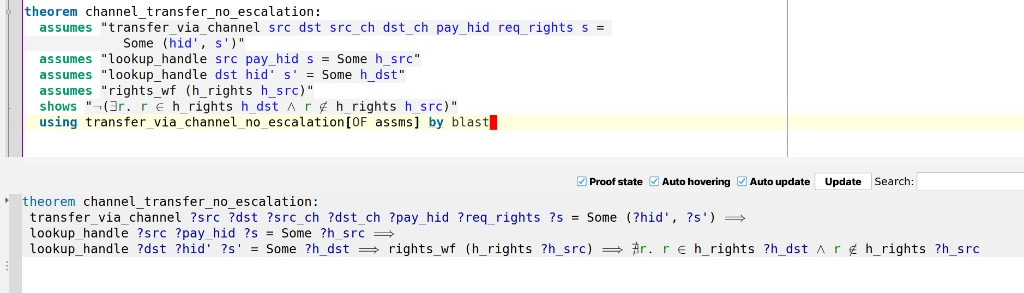
\includegraphics[width=\textwidth]{figures/isabelle-channel-transfer-no-escalation.png}
	\caption{Isabelle/jEdit (PIDE): формулировка
		\lemmaname{channel\_transfer\_no\_escalation} в буфере
		\texttt{Zircon.thy} и принятое утверждение в панели Output.
		Доказательство~--- \texttt{by~blast} из
		\lemmaname{transfer\_via\_channel\_no\_escalation};
		сокращение прав~--- замкнутое пересечение
		(\lemmaname{reduce\_rights\_wf}).
		Предпосылка \lemmaname{rights\_wf} у источника на снимке
		явная; в трассовых теоремах она выводится из
		\texttt{state\_wf}, а не из стража syscall'а.}
	\label{fig:pide-no-escalation}
\end{figure}

Теорема утверждает: после успешной передачи через канал у получателя
не существует права, отсутствовавшего у отправителя. В
\texttt{Zircon.thy} она выводится из
\lemmaname{transfer\_via\_channel\_no\_escalation} тактикой
\texttt{by~blast}~--- по сути это переформулировка
«$h\_rights\ h\_\mathit{dst} \subseteq h\_rights\ h\_\mathit{src}$»
в виде «не существует права у получателя вне источника».

Содержательная работа сделана в
\lemmaname{transfer\_via\_channel\_no\_escalation}: из успешной
передачи извлекается факт
$h\_rights\ h\_\mathit{dst} =
	\mathit{reduce\_rights\_wf}\;\mathit{req}\;h\_rights\ h\_\mathit{src}$
(лемма \lemmaname{transfer\_via\_channel\_cap}) и применяется
\lemmaname{reduce\_rights\_wf\_le\_old}, которое утверждает вложение

\[
	\mathit{reduce\_rights\_wf}\;\mathit{req}\;\mathit{src}
	\;\subseteq\;\mathit{src}
	\quad\text{при условии}\quad
	\lemmaname{rights\_wf}\;\mathit{src}.
\]

Оговорка про \lemmaname{rights\_wf} существенна: без неё лемма
неверна (замыкание могло~бы добавить \texttt{READ}). Syscall её не
проверяет; посылка берётся из \texttt{state\_wf}, а на трассах~---
извлекается в
\lemmaname{reachable\_transfer\_no\_escalation}
(\S\ref{sec:port-traces}). Развёрнутое разъяснение и контрпример
\lemmaname{transfer\_without\_wf\_source\_may\_escalate}~--- в~§3.1;
алгебраическая сторона~--- в~§8.5.1.

Итоговая цепочка

\[
	\underbrace{h\_rights\ h\_\mathit{dst}}_{\text{права получателя}}
	= \mathit{reduce\_rights\_wf}\;\mathit{req}\;h\_\mathit{src}
	\subseteq
	\underbrace{h\_rights\ h\_\mathit{src}}_{\text{права источника}}
\]

и есть то, что читает
\lemmaname{channel\_transfer\_no\_escalation}. Лемма
\lemmaname{transfer\_rights\_eq\_meet} из \texttt{Zircon\_Lattice.thy}
устанавливает то~же равенство на языке решёток (имя
\emph{meet}~--- отсылка к встрече; строгое
\lemmaname{reduce\_rights}$\,=\,$\texttt{inf}~--- в~§8.1), но
\emph{не} участвует в доказательстве теоремы ядра: теория решётки
импортирует \texttt{Zircon}, а не наоборот. Решёточные варианты~---
параллельная иллюстрация, а не основание главных security-лемм.

На рис.~\ref{fig:pide-no-escalation} видно, как PIDE отображает
формулировку в редакторе и в Output после успешной проверки. В отличие
от единичного тестового примера, утверждение относится ко всем
состояниям, удовлетворяющим предпосылкам модели.
Конкретная транзакция, разобранная в~§4 (\emph{Пошаговый разбор}), и
таблица~\ref{tab:write-guards} показывают, что у каждого из пяти
условий-стражей есть \emph{своя} лемма (или свой аспект семантики):
убрать страж~--- значит потерять именно её, а не обязательно
\lemmaname{channel\_transfer\_no\_escalation}. Например, без
$\mathit{req}\subseteq h\_rights$ no-escalation сохраняется
(пересечение не добавляет прав), но ломается соответствие
\texttt{ZX\_ERR\_INVALID\_ARGS}; без
\texttt{ch\_hid ≠ pay\_hid} лемма о move остаётся формально истинной,
хотя смысл self-move теряется. Успех самой
\lemmaname{channel\_transfer\_no\_escalation} наследует ещё и
ограничение композиции \lemmaname{transfer\_via\_channel}: очередь
получателя должна быть пуста (см.\ границу модели); у
\lemmaname{zx\_channel\_write} пустота не требуется.

\subsection{Дублирование дескриптора: тот~же meet}

Сокращение прав~--- это не только операция передачи по каналу. Тот же
приём используется в модели ещё раз, при дублировании дескриптора:
операция \lemmaname{zx\_handle\_duplicate} создаёт \emph{новый}
дескриптор на тот же объект ядра, но с урезанной маской. В реальном
Zircon такой вызов используется постоянно~--- например, когда один
сервис хочет дать другому только часть своих полномочий на объект,
не теряя собственный доступ. Свежий идентификатор дескриптора выделяет
\texttt{alloc\_hid}; исходный дескриптор при этом \emph{сохраняется},
то есть операция работает как копирование с ослаблением прав, а не как
передача:
\begin{lstlisting}
definition zx_handle_duplicate ::
  "process_id ⇒ handle_id ⇒ rights ⇒ system_state ⇒
   (handle_id × system_state) option" where
  "zx_handle_duplicate pid hid req_rights s =
    (case (lookup_handle pid hid s, get_table pid s) of
      (Some h, Some ht) ⇒
        if ZX_RIGHT_DUPLICATE ∉ h_rights h then None
        else if ¬ (req_rights ⊆ h_rights h) then None
        else
          (let actual = reduce_rights_wf req_rights (h_rights h);
               h' = h <| h_rights := actual |>;
               (hid', s1) = alloc_hid pid s
           in Some (hid', set_table pid (ht(hid' ↦ h')) s1))
    | _ ⇒ None)"
\end{lstlisting}
Лемма no-escalation для duplicate выписывается явно (тот~же meet +
\lemmaname{reduce\_rights\_wf\_le\_old}):
\begin{lstlisting}
lemma zx_handle_duplicate_no_escalation:
  assumes "zx_handle_duplicate pid hid req_rights s = Some (hid', s')"
      and "lookup_handle pid hid s = Some h"
      and "lookup_handle pid hid' s' = Some h'"
      and "rights_wf (h_rights h)"
  shows "h_rights h' ≤ h_rights h"
\end{lstlisting}
Предпосылка \lemmaname{rights\_wf}~--- как у канала (§3.1); трассовая
форма~--- \lemmaname{reachable\_duplicate\_no\_escalation}.
Рядом введён \lemmaname{zx\_handle\_close} (удаление слота): в
Zircon семантика \texttt{ZX\_HANDLE\_OP\_MOVE} у
\texttt{zx\_channel\_write\_etc} эквивалентна
\texttt{zx\_handle\_replace} с последующей записью; в модели move
встроен в \lemmaname{zx\_channel\_write}, а close оставлен явным (без
счётчика ссылок на объект~--- см. границу модели в начале статьи), чтобы
таблица дескрипторов была полнее для будущего refinement. Обе операции
есть и как метки трасс (\texttt{Duplicate}, \texttt{Close}), так что
\texttt{state\_wf} доказан сохраняющимся и через них. Методический вывод:
передающие операции (канал, duplicate)~--- это один и тот~же meet,
применённый к разным входам.

\section{Примерный сценарий}

Учебный сценарий задан прямо в теории: в \texttt{Zircon.thy} он
зафиксирован как замкнутый булев предикат \texttt{example\_scenario}
и \emph{принят} леммой \lemmaname{example\_scenario\_true}
(\texttt{"example\_scenario"}). Isabelle разворачивает определения
операций и проверяет конкретную трассу целиком~--- этого достаточно,
чтобы убедиться, что все определения согласованы между собой на
одном конкретном входе.

Подчеркнём эпистемический статус этого предиката. Лемма
\lemmaname{example\_scenario\_true}~--- это \emph{свидетель}
(конкретный пример, на котором модель ведёт себя ожидаемо), а не
универсальная теорема. Она не заменяет
\lemmaname{channel\_transfer\_no\_escalation}: та утверждает свойство
для \emph{всех} состояний с данными предпосылками, а сценарий~---
лишь для одного. Контрапозиция к \texttt{example\_scenario} была~бы
контрпримером к \emph{определениям} модели (или к самому сценарию),
а не опровержением универсальной теоремы.

По шагам предикат фиксирует:
\begin{enumerate}[leftmargin=1.4em]
	\item \lemmaname{create\_channel\_pair} выдаёт процессам~0 и~1 по handle
	      на два конца одного канала (пиры, связанные \texttt{channel\_peer});
	\item процесс~0 создаёт VMO с содержимым~42 и правами
	      \texttt{READ\,|\,WRITE\,|\,TRANSFER};
	\item дескриптор передаётся процессу~1 с запросом только
	      \texttt{READ} (move);
	\item у получателя есть \texttt{READ}, нет \texttt{WRITE}; у отправителя
	      payload-handle исчез;
	\item \texttt{vmo\_write} процесса~1 значения~99 возвращает \texttt{None};
	\item содержимое VMO остаётся~\texttt{Some~42}.
\end{enumerate}

\begin{lstlisting}
lemma example_scenario_true: "example_scenario"
  unfolding example_scenario_def ... by simp
\end{lstlisting}

Сценарий независим от конкретной аппаратной платформы и компилятора
ядра: он фиксирует свойство \emph{модели}, воспроизводимое при
пересборке теории. Тот~же смысл переносится в
исполняемый слой: \texttt{Zircon\_Code.thy} определяет
\lemmaname{example\_exec\_ok}, доказывает
\lemmaname{example\_exec\_ok\_true} и проверяет выражение через
\texttt{test\_code} / OCaml.

\section{Методические следствия}

\subsection{Раннее обнаружение архитектурных дефектов}

Ошибка спецификации вида "передача без проверки \texttt{TRANSFER}" в
реализационном коде может проявиться лишь в эксплуатации. В формальной
модели отсутствие соответствующей проверки препятствует доказательству
леммы \lemmaname{channel\_write\_requires\_transfer}: теория не
собирается, пока шлюз не восстановлен. Это и есть ранний сигнал
"архитектура небезопасна", даже если промышленный код ещё не написан.

\subsection{Оценка трудозатрат}

Для полной учебной Isabelle-сессии этой работы (см.\ глоссарий;
каналы с handles и move, решётка, зависимые права, трассы,
MMIO-контрпример, экстракция и \texttt{value}/\texttt{eval})
реалистичны следующие порядки:
\begin{itemize}[leftmargin=1.4em]
	\item в сопровождающем репозитории~--- порядка 2500 строк по шести
	      теориям сессии
	      (\texttt{Portable\_Capability.thy}, \texttt{Zircon.thy},
	      \texttt{Zircon\_Lattice.thy}, \texttt{Zircon\_Traces.thy},
	      \texttt{Zircon\_MMIO.thy}, \texttt{Zircon\_Code.thy};
	      \texttt{wc -l}, после правок peer/DUPLICATE/subset), из них
	      порядка двух третей~--- определения и сопровождающий текст,
	      остальное~--- леммы и доказательства;
	\item от нескольких дней до пары недель на построение, отладку
	      доказательств и настройку экстракции~--- в зависимости от опыта
	      с Isabelle;
	\item Isabelle/HOL как свободно распространяемый инструмент с
	      документацией.
\end{itemize}
Это всё ещё \emph{на порядки} меньше промышленного порта драйвера или
полного syscall surface, но уже не «сотня строк за вечер»: читатель,
воспроизводящий модель, должен ожидать объём курса/мини-проекта, а не
лабораторной заготовки на час. Формализация отвечает на вопрос об
инварианте делегирования прав, который можно зафиксировать локально и
относительно дёшево по сравнению с полным портом железа~--- но не
бесплатно.

\paragraph{Масштаб для сравнения.}
Порядок приведённых цифр стоит сопоставить с масштабом полной
верификации: проект seL4 потребовал порядка двух десятков
человеко-лет и сотен тысяч строк скриптов Isabelle/HOL
\cite{sel4overview}. Наша заметка не конкурирует с этим масштабом~---
она показывает, что проверка \emph{архитектурных} инвариантов
делегирования возможна на порядки дешевле и на порядки \emph{раньше},
чем полная верификация. Именно эта «ранняя» роль микромодели нас здесь
и интересует: отвергнуть небезопасную архитектуру до того, как в неё
вложены человеко-годы.

\subsection{Соотношение с тестированием и фаззингом}

Формальная проверка инвариантов не заменяет эмпирические методы, а
дополняет их иным классом гарантий. Табл.~\ref{tab:compare} сводит
четыре свойства, по которым эти классы различаются.

\begin{table}[ht]
	\centering
	\caption{Сопоставление методов обеспечения качества для инварианта
		отсутствия эскалации прав.}
	\label{tab:compare}
	\begin{tabular}{@{}lccc@{}}
		\toprule
		\textbf{Свойство}                    &
		\textbf{Тесты}                       &
		\textbf{Фаззинг}                     &
		\textbf{Форм.\ вер.}                                  \\
		\midrule
		Доказанное отсутствие эскалации      &
		---                                  & --- & да       \\
		Общность по состояниям модели        &
		---                                  & --- & да       \\
		Автоматизированная проверка          &
		да                                   & да  & да       \\
		Быстрое обнаружение частных дефектов &
		да                                   & да  & частично \\
		\bottomrule
	\end{tabular}
\end{table}

Два верхних свойства~--- «доказанное отсутствие эскалации» и «общность
по состояниям модели»~--- принципиально недостижимы ни тестированием,
ни фаззингом. Тест проверяет поведение на конкретных входах; он не
может перебрать все допустимые состояния и не может установить
свойство вида «для всех~$s$». Фаззинг идёт дальше в смысле охвата
входов, но сам по себе остаётся эмпирическим: успешный прогон
фаззера не доказывает отсутствия дефекта, он лишь не нашёл его за
отведённое время.

Автоматизированная проверка у всех трёх методов есть, но её природа
различна. У тестов и фаззера это прогон на наборе входов; у
формальной верификации~--- сборка теории Isabelle, где каждая тактика
либо завершается успешно, либо падает. Именно последнее свойство
делает вклад формального метода уникальным: успешная сборка теории не
оставляет возможности «не заметить» контрпример, тогда как успешный
тест или фаззер всегда допускает, что нужный вход просто не был
предъявлен.

Быстрое обнаружение частных дефектов~--- сильная сторона тестов и
фаззинга и лишь частичная~--- формальной верификации. Доказательство
не заменяет модульный тест: если ошибка лежит \emph{вне} формальной
модели (например, в кодогенераторе или в обработке пользовательского
ввода), Isabelle её не увидит. Формальная верификация и эмпирические
методы~--- не конкуренты, а разные инструменты одного процесса
обеспечения качества.

\section{Алгебраическая структура прав: решётка}

До сих пор права трактовались как множества, а сокращение~--- как
пересечение. За этой операцией стоит стандартная алгебраическая
структура: семейство всех подмножеств атомарных флагов с операциями
$\cap$ и $\cup$ образует \emph{дистрибутивную решётку}
(distributive lattice).

Стоит сразу оговорить статус равенства
\lemmaname{reduce\_rights}\,$=\,$\texttt{inf}. Это \emph{наше}
определение~--- технический приём, облегчающий доказательство, а не
«открытие о природе Zircon». Сокращение прав можно было~бы определить
и пересечением с учётом приоритетов, и сужением по маске, и любой
другой монотонной операцией; определения системных вызовов остались
бы осмысленными. Но именно пересечение даёт самые короткие
машинно проверяемые выводы, поскольку опирается на уже встроенную в
HOL алгебру на \texttt{'a~set}. В Isabelle/HOL эта структура доступна для
типа \texttt{'a~set} (следовательно, и для \texttt{rights}) через
классы \texttt{semilattice\_inf}/\texttt{semilattice\_sup}, \texttt{lattice} и
\texttt{distrib\_lattice} теории \texttt{Main}
(см.~также~\cite{nipkowklein,isabelle}).

Поскольку тип \texttt{rights} является синонимом для \texttt{set~right},
все операции решётки (\texttt{inf}, \texttt{sup}, $\le$) доступны
автоматически. Отдельный \texttt{instantiation} для синонима типа
невозможен и не нужен: мы явно фиксируем равенство
\lemmaname{reduce\_rights}\,$=\,$\texttt{inf} и выводим свойства модели
как следствия законов решёток (при желании тот же смысл можно оформить
через \texttt{interpretation}, но для данной работы достаточно прямого
равенства).

\subsection{Права как решётка}

Встреча (meet; в Isabelle~--- \texttt{inf}, теоретико-множественно~---
пересечение~$\cap$) на множествах прав совпадает с~$\cap$; соединение
(join; \texttt{sup}, объединение~$\cup$)~--- с~$\cup$. Тем самым
автоматически выполняются коммутативность, ассоциативность,
идемпотентность и законы поглощения. Ниже в формулах для сокращения прав
используем именно~$\cap$~/~\texttt{inf} (встречу), а не~$\cup$~/~\texttt{sup}
(соединение).

В теории \texttt{Zircon\_Lattice} это фиксируется равенством
\begin{lstlisting}
lemma reduce_rights_eq_inf:
  "reduce_rights new_rights old_rights = inf new_rights old_rights"
  by (simp add: reduce_rights_def)
\end{lstlisting}
и следствиями
\begin{lstlisting}
lemma reduce_rights_commute:
  "reduce_rights A B = reduce_rights B A"
  by (simp add: reduce_rights_eq_inf inf_commute)

lemma reduce_rights_assoc_via_lattice:
  "reduce_rights R1 (reduce_rights R2 R) =
     reduce_rights (inf R1 R2) R"
  by (simp add: reduce_rights_eq_inf inf_assoc)
\end{lstlisting}
Последнее утверждение~--- ассоциативность цепочки сокращений
(ассоциативность встречи), а не идемпотентность; идемпотентность
\texttt{inf} формулируется отдельно (\texttt{reduce\_rights A A = A}).

\subsection{Частичный порядок}

Порядок на правах совпадает с включением: $A \le B$ означает
$A \subseteq B$. Пустое множество~--- наименьший элемент $\bot$;
\texttt{UNIV} (полный набор флагов типа \texttt{right})~--- наибольший
элемент $\top$ в данной модели. «Уменьшение прав» при передаче~---
переход к элементу, меньшему или равному исходному в этом порядке.

\begin{lstlisting}
lemma reduce_rights_le_old:
  "reduce_rights new_rights old_rights ≤ old_rights"
  by (simp add: reduce_rights_eq_inf)

lemma reduce_rights_greatest:
  assumes "C ≤ new_rights" "C ≤ old_rights"
  shows "C ≤ reduce_rights new_rights old_rights"
  using assms by (simp add: reduce_rights_eq_inf)
\end{lstlisting}
Вторая лемма выражает характеризацию встречи как \emph{наибольшей
	нижней грани} (greatest lower bound)~--- то есть как самого «щедрого»
из допустимых результатов.

Развернём это человеческим языком. Пусть даны два ограничения: набор
прав не должен выходить за запрос и не должен выходить за источник.
Среди всех наборов, которые одновременно удовлетворяют обоим
ограничениям, существует наибольший~--- и это в точности результат
сокращения. Любой другой набор, подходящий под оба ограничения,
вложен в него. Именно поэтому модель не «урезает права сверх
необходимого»: она возвращает максимум из допустимого.

\subsection{Переформулировка свойств безопасности}

\paragraph{Отсутствие эскалации.}
Закон $\mathit{inf}(a,b)\le b$ (эквивалентно $a\cap b\subseteq b$)
непосредственно даёт: результат сокращения не содержит прав вне исходного
набора.
\begin{lstlisting}
lemma no_escalation_via_meet:
  "¬(∃r. r ∈ reduce_rights req src ∧ r ∉ src)"
  using reduce_rights_le_old[of req src]
  by (auto simp: reduce_rights_def)
\end{lstlisting}

\paragraph{Передача как встреча с замыканием.}
Для успешного \lemmaname{transfer\_via\_channel} права получателя в точности
равны \emph{встрече запроса и прав отправителя с последующим замыканием
	зависимостей}~--- то есть \lemmaname{reduce\_rights\_wf}, а не сырому
\texttt{inf}:
\begin{lstlisting}
lemma transfer_rights_eq_meet:
  assumes "transfer_via_channel ... = Some (hid', s')"
      and "lookup_handle src pay_hid s = Some h_src"
      and "lookup_handle dst hid' s' = Some h_dst"
  shows "h_rights h_dst =
           reduce_rights_wf req_rights (h_rights h_src)"
\end{lstlisting}
Отсюда
\begin{lstlisting}
theorem channel_transfer_no_escalation_via_lattice:
  ...
  shows "h_rights h_dst ≤ h_rights h_src"

theorem channel_transfer_respects_request_via_lattice:
  ...
  shows "h_rights h_dst ≤ close_rights req_rights"
\end{lstlisting}
то есть одновременно $R_{\mathrm{dst}} \le R_{\mathrm{src}}$ и
$R_{\mathrm{dst}} \le \mathit{close}(R_{\mathrm{req}})$ (замыкание
запроса~--- верхняя оценка после \lemmaname{reduce\_rights\_wf}).

\paragraph{Монотонность по отправителю.}
Расширение прав отправителя не уменьшает результат при фиксированном
запросе (монотонность \texttt{inf} по одному аргументу):
\begin{lstlisting}
lemma reduce_rights_mono_old:
  assumes "old_rights ≤ old_rights'"
  shows "reduce_rights req old_rights ≤
           reduce_rights req old_rights'"
  using assms by (auto simp: reduce_rights_eq_inf)
\end{lstlisting}

\subsection{Соединение (join) и агрегация прав}

Передача \textenglish{capability} опирается на \emph{встречу}. Для сценариев слияния
(наследование, объединение пространств имён) нужна двойственная операция
соединения:
\begin{lstlisting}
definition combine_rights :: "rights ⇒ rights ⇒ rights" where
  "combine_rights A B = (A ∪ B)"   (* = sup *)

lemma combine_rights_ge_left:  "A ≤ combine_rights A B"
lemma combine_rights_ge_right: "B ≤ combine_rights A B"
lemma combine_may_exceed_left:
  "¬ (combine_rights {} {ZX_RIGHT_READ} ≤ {})"
\end{lstlisting}
Здесь $\{\}$~--- нижний элемент решётки $\bot$ (пустой набор флагов как
элемент порядка), а не «handle с пустой маской в смысле~§3.2»; лемма
лишь показывает, что join может выйти за левый аргумент. Join~---
наименьшая верхняя грань, но \emph{не} закон no-escalation
относительно одного родителя: результат может превосходить каждый из
аргументов. Дистрибутивность решётки даёт
\begin{lstlisting}
lemma reduce_rights_distrib_join:
  "reduce_rights (combine_rights A B) C =
     combine_rights (reduce_rights A C) (reduce_rights B C)"
\end{lstlisting}
то есть сокращение агрегата~--- агрегат сокращений.

\subsection{Зависимые права}

Минимальная учебная зависимость: наличие \texttt{WRITE} или
\texttt{EXECUTE} влечёт \texttt{READ}. Это фиксируется определением
\begin{lstlisting}
definition rights_wf :: "rights ⇒ bool" where
  "rights_wf R ≡
     (ZX_RIGHT_WRITE ∈ R ⟶ ZX_RIGHT_READ ∈ R) ∧
     (ZX_RIGHT_EXECUTE ∈ R ⟶ ZX_RIGHT_READ ∈ R)"
\end{lstlisting}
Предикат \lemmaname{close\_rights} замыкает маску по зависимостям
(добавляет \texttt{READ}, если есть \texttt{WRITE}/\texttt{EXECUTE}).
Само замыкание идемпотентно всюду
(\texttt{close\_rights (close\_rights R) = close\_rights R}); лемма
ниже~--- иное свойство: она \emph{характеризует корректные маски как
	неподвижные точки} \lemmaname{close\_rights}:
\begin{lstlisting}
lemma close_rights_idem:
  "close_rights (close_rights R) = close_rights R"

lemma close_rights_fix_wf:
  "rights_wf R ⟷ close_rights R = R"
\end{lstlisting}
Определения \lemmaname{close\_rights}/\lemmaname{rights\_wf} и обе леммы
живут в \texttt{Zircon.thy}; здесь, в решёточном разделе, они
\emph{используются} как мост к \lemmaname{reduce\_rights\_wf}.

\paragraph{Оговорка о реализме.}
В настоящем Zircon права \texttt{ZX\_RIGHT\_READ} и
\texttt{ZX\_RIGHT\_WRITE} \emph{независимы}: handle может позволять
запись без чтения, и наоборот. Зависимость
$\texttt{WRITE} \Rightarrow \texttt{READ}$ введена здесь
\emph{искусственно}~--- как минимальный пример, на котором видно,
зачем нужен отдельный шаг замыкания \lemmaname{close\_rights} поверх
сырого пересечения. Это не разрешение «раз есть \texttt{WRITE}, можно
выдать и \texttt{READ}»: замыкание \emph{копирует} бит, который у
корректного источника уже был, и только поэтому не ломает no-escalation.
Читатель, работающий с другим ядром, может заменить
эту зависимость на любую другую (например,
$\texttt{EXECUTE} \Rightarrow \texttt{MAP} \Rightarrow \texttt{READ}$,
см.~§8.5.1) или на пустое отношение~--- в последнем случае
$\mathit{close} = \mathit{id}$, и три аксиомы замыкания тривиальны.
Структура доказательств не меняется.

\subsubsection{Ключевая лемма: почему замыкание не нарушает
	no-escalation}

Сырое пересечение может нарушить зависимости:
\begin{lstlisting}
lemma reduce_rights_may_break_wf:
  "rights_wf {READ, WRITE} ∧
   ¬ rights_wf (reduce_rights {WRITE} {READ, WRITE})"

definition reduce_rights_wf where
  "reduce_rights_wf req src = close_rights (reduce_rights req src)"
\end{lstlisting}
\lemmaname{close\_rights} формально \emph{добавляет} \texttt{READ} к
маске. Казалось~бы, это эскалация относительно голого meet. Главная
лемма раздела снимает кажущийся парадокс:
\begin{lstlisting}
lemma reduce_rights_wf_le_old:
  assumes "rights_wf src"
  shows "reduce_rights_wf req src ≤ src"
\end{lstlisting}
Она говорит не «no-escalation через meet» (это следствует из
\texttt{inf}~$\le$~аргумента), а сильнее по смыслу для модели с
зависимостями: \emph{no-escalation несмотря на замыкание}. Добавленные
замыканием флаги уже обязаны быть в \texttt{src}, иначе источник не
удовлетворял~бы \texttt{rights\_wf}. Получатель видит \texttt{READ} рядом
с \texttt{WRITE} не потому, что модель дарит чтение, а потому, что у
источника оно уже было.

Разделим два мотива. \emph{Зачем} \lemmaname{reduce\_rights\_wf}, а не
сырое пересечение: результат замыкания всегда удовлетворяет
\lemmaname{rights\_wf} (\lemmaname{close\_rights\_wf}), так что в очередь
не попадёт «сломанная» маска. \emph{Зачем} предпосылка
\lemmaname{rights\_wf} у источника: без неё замыкание может
\emph{добавить} \texttt{READ}, которого в источнике не было~--- и
сломать no-escalation, хотя маска получателя останется корректной.
Для самой леммы \lemmaname{reduce\_rights\_wf\_le\_old} в доказательстве
достаточно монотонности \texttt{close} и одной стороны
\texttt{close\_fix\_wf} ($\mathit{wf}\Rightarrow\mathit{close}=\mathit{id}$);
идемпотентность нужна для алгебры замыкания в целом, а не как
единственная опора этой леммы. Закрытие~--- бухгалтерия зависимостей,
а не послабление политики. Именно к
\lemmaname{reduce\_rights\_wf\_le\_old} придётся вернуться, добавляя
новые рёбра зависимостей (например, \texttt{EXECUTE}$\Rightarrow$\texttt{MAP}$\Rightarrow$\texttt{READ}).
В~\S\ref{sec:port-locale} та~же лемма появляется как следствие locale
\texttt{portable\_capability}: «парадокс» исчезает, когда замыкание
задано аксиомами монотонности, инфляции и неподвижных точек.

Лемма \lemmaname{reduce\_rights\_may\_break\_wf}~--- мотивация введения
замыкания, а не «баг модели». В syscall-пути
\lemmaname{zx\_channel\_write} и \lemmaname{zx\_handle\_duplicate}
используют \lemmaname{reduce\_rights\_wf}; \lemmaname{rights\_wf} у
источника~--- из \texttt{state\_wf}, а не из стража syscall'а
(канон~--- §3.1). Явная проверка \lemmaname{rights\_wf}~--- только в
\texttt{create\_vmo} / \texttt{create\_channel\_pair}.

\subsection{Алгебраический разбор сценария}

Для $R_{\mathrm{src}}=\{\mathtt{READ},\mathtt{WRITE},\mathtt{TRANSFER}\}$ и
$R_{\mathrm{req}}=\{\mathtt{READ}\}$ результат~--- \emph{встреча} (meet /
\texttt{inf} / $\cap$), а не соединение (join / $\cup$):
\[
	R_{\mathrm{dst}}
	= R_{\mathrm{src}} \cap R_{\mathrm{req}}
	= \{\mathtt{READ}\}.
\]
В этом частном случае замыкание не срабатывает:
\lemmaname{reduce\_rights\_wf} совпадает с \lemmaname{reduce\_rights},
потому что \{\texttt{READ}\} уже содержит \texttt{READ}. Различие с
\S~о зависимых правах видно на запросе \{\texttt{WRITE}\} против того~же
источника: сырое пересечение даёт \{\texttt{WRITE}\}, а
\lemmaname{reduce\_rights\_wf}~--- \{\texttt{READ},\texttt{WRITE}\}
(см.~также \texttt{value}/\texttt{eval} в разделе экстракции).
Машинно для «чистой» встречи:
\begin{lstlisting}
lemma example_meet_computation:
  "reduce_rights {ZX_RIGHT_READ}
      {ZX_RIGHT_READ, ZX_RIGHT_WRITE, ZX_RIGHT_TRANSFER}
   = {ZX_RIGHT_READ}"
  by (simp add: reduce_rights_def)
\end{lstlisting}
Свойство наибольшей нижней грани объясняет, почему модель не «урезает
права сверх необходимого»: среди всех наборов, допустимых и запросом, и
исходной маской, выбирается наибольший.

\subsection{Методический эффект решёточной абстракции}

Как видно из табл.~\ref{tab:lattice}, решёточный подход меняет не только
формулировки, но и способ переиспользования доказательств: вместо
изолированных рассуждений о $\cap$ появляются следствия уже встроенной в
HOL алгебры.

\begin{table}[ht]
	\centering
	\caption{Сопоставление формулировок без явной решётки и с опорой на неё.}
	\label{tab:lattice}
	\begin{tabular}{@{}p{0.22\textwidth}p{0.33\textwidth}p{0.33\textwidth}@{}}
		\toprule
		\textbf{Аспект}                 &
		\textbf{Без решётки}            &
		\textbf{С решёткой}                    \\
		\midrule
		Язык свойств                    &
		операции на множествах          &
		законы \texttt{inf}/\texttt{sup}/$\le$ \\
		Доказательства                  &
		отдельные леммы о $\cap$        &
		следствия классов HOL                  \\
		Масштабирование                 &
		каждое свойство заново          &
		наследование алгебры                   \\
		Интерпретация передачи          &
		«пересечение не добавляет прав» &
		«передача~--- встреча в решётке»       \\
		Расширение набора прав          &
		новые флаги требуют ручной
		проверки всех лемм              &
		новые атомы прав наследуют
		законы \texttt{inf}/\texttt{sup}
		(гипотетически; в модели их нет)       \\
		\bottomrule
	\end{tabular}
\end{table}

Аппарат решёток не отменяет конкретные леммы о каналах и VMO, а
поднимает их на уровень, где «нет эскалации» читается как частный случай
монотонности и свойства нижней грани~--- хорошо изученных фактов
универсальной алгебры, уже встроенных в Isabelle/HOL.

\section{Контрпример MMIO: когда шлюз \textenglish{capability} недостаточен}

Индустриальный конфликт «безопасность vs совместимость» (драйверы модема,
Starnix-подобные слои) формализуется не расширением списка «хороших»
syscall, а явным \emph{обходом}. Важно: это \emph{гипотетический}
немедиируемый poke, а не модель реального пути Fuchsia, где MMIO
выдаётся через ресурс \texttt{ZX\_RSRC\_KIND\_MMIO} и физический VMO.
Теория \texttt{Zircon\_MMIO.thy} вводит
привилегированную запись в \texttt{vmo\_store} по сырому
\texttt{obj\_id}~--- без \texttt{lookup\_handle} и без проверки
\texttt{WRITE}. В модели поле \texttt{vmo\_store} имеет тип
\texttt{obj\_id $\rightharpoonup$ nat}: содержимое адресуется идентификатором
объекта, а не handle; обычный \lemmaname{vmo\_write} сначала решает
\texttt{obj\_id} через таблицу дескрипторов, poke~--- нет (снова
\texttt{<|...|>} вместо Isabelle record-update):
\begin{lstlisting}
definition privileged_vmo_poke ::
  "obj_id ⇒ nat ⇒ system_state ⇒ system_state" where
  "privileged_vmo_poke oid content s =
     s <| vmo_store := (vmo_store s)(oid ↦ content) |>"
\end{lstlisting}
В отличие от \lemmaname{vmo\_write}, переход никогда не возвращает
\texttt{None}: нет handle, нет типовой проверки, нет маски прав.

Свидетель \lemmaname{mmio\_leak\_witness}~--- булев предикат в том~же
стиле, что и \lemmaname{example\_scenario}: учебный путь (канал, VMO~42,
передача только \texttt{READ}), отказ \texttt{vmo\_write} у получателя,
затем привилегированный poke, меняющий содержимое на~99 при всё ещё
отсутствующем \texttt{WRITE}:
\begin{lstlisting}
definition mmio_leak_witness :: bool where
  "mmio_leak_witness =
    (... create_channel_pair; create_vmo 0 ... 42;
         transfer_via_channel ... {ZX_RIGHT_READ} ...;
     case lookup_handle 1 hid_b s3 of
       Some h_b ⇒
         ZX_RIGHT_WRITE ∉ h_rights h_b ∧
         vmo_write 1 hid_b 99 s3 = None ∧
         vmo_content oid s3 = Some 42 ∧
         (let s4 = privileged_vmo_poke oid 99 s3
          in vmo_content oid s4 = Some 99 ∧
             lookup_handle 1 hid_b s4 = Some h_b ∧
             ZX_RIGHT_WRITE ∉ h_rights h_b)
     | _ ⇒ False)"

lemma mmio_leak_witness_true: "mmio_leak_witness"
\end{lstlisting}
Лемма лишь принимает этот предикат (\texttt{by~simp} после разворачивания
определений). Архитектурное чтение: леммы \textenglish{capability}-IPC при
этом \emph{не опровергнуты}~--- они по-прежнему истинны для опосредованных
переходов. Опровергнуто системное утверждение вида «store меняется только
через \texttt{vmo\_write}»: достаточно добавить один неперехватываемый
путь, и изоляция по маске перестаёт быть свойством всей системы. Именно
такова форма компромисса «открыть MMIO спец-syscall'ом» из
индустриального контекста выше.

\paragraph{Разные эпистемологии: witness vs отсутствие обходов.}
Подход seL4 к обходам~--- \emph{доказать их отсутствие}: инварианты
политики сохраняются на всём стеке refinement, включая обработчики
прерываний и управление таблицами страниц
\cite{sel4overview}. Мы используем двойственный приём: не доказываем
отсутствие обходов, а предъявляем конкретный обход как \emph{negative witness}
(негативный свидетель, контрпример к утверждению)
(\lemmaname{mmio\_leak\_witness\_true}).
Разница принципиальна. Доказательство отсутствия обходов требует
полной модели железа, обработчиков прерываний и DMA (в Zircon доступ к
MMIO выдаётся через ресурс \texttt{ZX\_RSRC\_KIND\_MMIO}, а DMA
ограничивается IOMMU через bus transaction initiator, BTI)~--- то есть
работы масштаба seL4. Negative witness требует лишь одной строчки, описывающей
обход, и одного доказательства, что он ломает конкретный инвариант.
Именно поэтому negative witness~--- реалистичный инструмент
\emph{ранней} аттестации архитектуры, тогда как полное доказательство
отсутствия обходов~--- задача уровня сертификации ядра.

\section{От модели к коду: проблематика refinement}

Доказанные леммы живут в мире \emph{абстрактных} переходов
$s\mapsto\texttt{Some}~s'$. Читатель, привыкший к промышленным ядрам,
закономерно спрашивает: что связывает эту картину с тысячами строк C++ в
Zircon, с гонками на таблицах дескрипторов, с оптимизациями компилятора и
с драйверами, которые «просто пишут в регистр»? Ответ не в расширении
списка syscall на всё ядро~--- для обзорной статьи это непосильный и
методологически чуждый шаг,~--- а в понятии \emph{уточнения}
(refinement): отношения между слоями описания одной и той~же системы.

Здесь важно не смешивать два разных желания. Первое~--- \emph{покрыть
	больше API}: добавить порты, события, полный набор rights, планировщик.
Второе~--- \emph{спуститься ближе к коду}, который действительно
исполняется. Первое увеличивает ширину модели; второе~--- глубину доверия.
Обзорная работа сознательно выбирает глубину: лучше честно объяснить, чего
ещё нет между HOL-переходом и машинной инструкцией, чем обещать «ещё
немного syscall~--- и мы у верифицированного ядра».

\subsection{Три этажа одной башни}

Удобно мыслить три этажа~--- не как иерархию важности, а как уровни
\emph{наблюдаемости} одного и того~же замысла.
\begin{enumerate}[leftmargin=1.4em]
	\item \textbf{Политика / модель} (наш Isabelle/HOL).
	      Здесь формулируются объекты, операции и инварианты:
	      no-escalation, move, \texttt{rights\_wf}, сохранение
	      \texttt{state\_wf} на трассах, контрпример MMIO.
	      Язык~--- математика с исполняемыми определениями; ошибки здесь
	      стоят дешево и ловятся доказательством.
	\item \textbf{Исполняемая спецификация}.
	      Та же семантика, но уже не в виде математических утверждений,
	      а в виде \emph{программы}: её можно запустить и получить
	      результат. На практике это либо автоматическая экстракция в
	      язык программирования~--- в нашем случае в OCaml (см.~§11),~---
	      либо рукописный эталонный модуль на функциональном языке.
	      На этом уровне сценарии можно \emph{вычислять}
	      (\texttt{value}, \texttt{eval}, \texttt{test\_code}) и сравнивать
	      результаты с тем, что утверждают леммы. Это ещё не ядро~---
	      нет ни планировщика, ни работы с железом,~--- но и не «чистая
	      бумага»: у кода появляются типы целевого языка, порядок
	      вычислений и границы модулей. Именно здесь модель превращается
	      в артефакт, который инженер может запустить у себя на машине.
	\item \textbf{Код ядра} (C/C++ Zircon, ассемблерные вставки, DMA~---
	      прямой доступ устройств к памяти). Именно он исполняется на
	      железе. Между вторым и третьим этажом пролегает пропасть:
	      указатели, алиасинг (несколько ссылок на одну память), прерывания,
	      модель памяти, \emph{ABI} системных вызовов (двоичный интерфейс,
	      через который пользовательский код вызывает ядро), взаимодействие
	      с драйверами.
\end{enumerate}
Refinement~--- дисциплина, которая делает эту пропасть \emph{явной} и
частично устранимой: каждое поведение нижнего этажа должно быть
допустимым поведением верхнего (или наоборот~--- в зависимости от
выбранного направления симуляции). Пока отношение не установлено, фраза
«мы доказали безопасность \textenglish{capability}-IPC» относится строго к этажу~1.
Она не ложна~--- она \emph{узка}: истинна для модели, молчит о бинарнике.

Можно представить башню иначе: этаж~1 говорит, \emph{что разрешено};
этаж~2~--- \emph{как это считается} в идеализированной машине; этаж~3~---
\emph{что происходит} на реальном процессоре. Уточнение~--- договор о том,
что нижние этажи не изобретают лишних историй сверх разрешённых верхними.

\paragraph{Refinement как промышленная дисциплина.}
Классическая схема refinement в seL4 \cite{sel4overview} содержит
именно эти уровни~--- абстрактная спецификация, исполняемая
monadic-спецификация, C-код и, наконец, бинарник~--- и доказывает
симуляцию между каждой парой соседних уровней. Наша модель остаётся
на верхнем этаже: мы формулируем политику, доказываем её свойства и
останавливаемся. Ссылка на seL4 здесь нужна не для того, чтобы
присвоить себе часть её результата, а чтобы читатель видел:
«башня»~--- не авторская метафора, а редуцированная версия
промышленного фреймворка. Уровни, которые мы \emph{не} проходим,
перечислены явно; цена их прохождения~--- тоже.

\subsection{Что именно обещает уточнение}

Классическая схема (в духе проектов seL4~\cite{sel4}, CertiKOS, частей
Verve) звучит
так: если реализация $C$ \emph{уточняет} спецификацию
$S$ (refinement, доказанная \emph{симуляция}: каждое поведение $C$
допустимо как поведение $S$), а в $S$ доказан инвариант $I$, то $I$
переносится на $C$~--- при условии, что уточнение сохраняет
\emph{наблюдаемое поведение}, интересное для $I$, то есть все
свойства, которые мы умеем проверять на уровне $C$. Например, наблюдение
$h\_\mathit{rights}(h_{\mathrm{dst}}) \le h\_\mathit{rights}(h_{\mathrm{src}})$
должно быть выражено через \emph{наблюдаемые} поля состояния в~$C$
(биты в таблице дескрипторов ядра), а не через абстрактные
\texttt{h\_rights} модели~$S$. Для нашей модели это означало~бы, например:
\begin{itemize}[leftmargin=1.4em]
	\item успешный \texttt{zx\_channel\_write} в ядре не выдаёт получателю
	      прав сверх пересечения запроса и маски отправителя;
	\item move действительно удаляет локальный дескриптор отправителя;
	\item запись в VMO без \texttt{WRITE} в опосредованном syscall невозможна.
\end{itemize}
Без refinement те~же утверждения остаются \emph{гипотезами о коде},
подкреплёнными лишь тестами и код-ревью. С refinement они становятся
следствием доказанной симуляции~--- ценой огромной инженерной работы:
выбор представления состояния, доказательство шагов симуляции, учёт
ошибочных путей, иногда~--- переписывание кода «под доказательство».

Есть и обратная сторона обещания. Refinement не делает модель богаче:
он переносит \emph{уже доказанное}. Если в модели нет гонок, уточнение
не докажет их отсутствие в ядре~--- оно лишь потребует, чтобы
конкурентность либо была добавлена в $S$, либо исключена допущениями
(«последовательное исполнение», «один поток владеет таблицей»). Честность
refinement начинается с честности допущений.

\subsection{Почему это трудно именно для микроядра}

Микроядро Zircon~--- не идеальный объект для «полного seL4-стиля» в рамках
статьи. Код написан с расчётом на производительность и совместимость:
сложные структуры данных, ручное управление памятью, взаимодействие с
драйверами и слоями вроде Starnix. Формальный refinement требует либо
существенной \emph{перестройки} кода под доказательство (как в seL4), либо
инструментов, натягивающих логику на существующий C
(AutoCorres~\cite{autocorres}, VST~\cite{vst} и др.~--- инструменты,
позволяющие доказывать свойства C-кода, не переписывая его целиком на
функциональный язык), либо сужения цели до крошечного фрагмента.

Кроме того, сам объект уточнения нужно выбрать честно. Уточнять «всё
ядро» к учебной модели бессмысленно: модель намеренно беднее
(нет полного набора rights, нет конкуренции, MMIO введён как
контрпример, а не как полная модель железа). Имеет смысл говорить о
refinement \emph{вырезки}: например, путь
\texttt{channel\_write}/\texttt{read} + \texttt{vmo\_write} в изоляции,
на последовательном исполнении, с явно оговорёнными допущениями о памяти.

Именно здесь MMIO-контрпример из теории \texttt{Zircon\_MMIO} играет
методическую роль: он напоминает, что даже идеальный IPC-путь не спасает,
если рядом существует обход через привилегированную запись в ту~же
память. Refinement «только syscall» молчит о таких обходах, пока они не
включены в отношение наблюдаемости. Поэтому горизонт уточнения~--- не
лозунг «докажем всё ядро», а аккуратный выбор \emph{какие} наблюдения
мы считаем релевантными для переноса инварианта.

\subsection{Место экстракции на пути к refinement}

Экстракция Isabelle~$\to$~OCaml не заменяет refinement к Zircon. Она решает
другую, более скромную, но методически важную задачу: показывает, что
определения модели \emph{исполнимы} и что конкретные сценарии
(\lemmaname{example\_scenario}, пустая маска, алгебра
\lemmaname{reduce\_rights\_wf}) дают ожидаемые значения не только в
доказательстве \texttt{by~simp}, но и при вычислении кодогенератором.
Это~--- мост между этажами~1 и~2. Мост между этажами~2 и~3 остаётся
отдельным исследовательским проектом; в обзорной работе достаточно ясно
обозначить его цену и обещание, не имитируя завершённость.

Практический смысл такого моста для читателя-практика прост. Пока
утверждение живёт только как лемма, легко заподозрить «магию тактик».
Когда то~же утверждение печатается как \texttt{True} командой
\texttt{value~[code]}, а затем подтверждается внешним OCaml, подозрение
смещается: либо модель действительно считает так, либо ошибка общая для
доказательства и генератора~--- и тогда её ловят расхождением с
интуицией сценария. Это ещё не доказательство корректности ядра, но уже
\emph{воспроизводимый эксперимент} над спецификацией.

Иными словами: ниже мы спускаемся на этаж исполняемой спецификации и
проверяем утверждения вычислением. Читатель при этом помнит, что до
промышленного ядра ещё один~--- самый трудный~--- пролёт лестницы.

\section{От доказательств к исполняемому коду}

Формальные доказательства в Isabelle/HOL устанавливают свойства
\emph{модели}. Следующий шаг~--- связать их с исполняемой программой
\emph{той~же} семантики (этаж~2 выше), не претендуя ещё на бинарный
Zircon. Isabelle предоставляет генератор кода, транслирующий подходящие
спецификации в OCaml, Haskell, SML или Scala, а также команды
\texttt{value} и \texttt{eval} для проверки конкретных выражений.

\subsection{Принцип генерации}

Используется мелкое встраивание (\emph{shallow embedding}): логические
константы и типы отображаются напрямую на сущности целевого языка
(натуральные числа, множества, записи), без промежуточной модели
синтаксиса. Сгенерированная программа реализует систему переписывания
терминов; каждый шаг вычисления допускает \emph{симуляцию} в логике
(доказательство того, что конкретный результат кодогенератора
соответствует формальному определению), что обеспечивает частичную
корректность экстракции относительно выбранной спецификации кода.

В рассматриваемой модели автоматически транслируются, в частности,
\lemmaname{create\_vmo}, \lemmaname{zx\_channel\_write},
\lemmaname{zx\_channel\_read}, \lemmaname{transfer\_via\_channel},
\lemmaname{zx\_handle\_duplicate}, \lemmaname{zx\_handle\_close} и
\lemmaname{vmo\_write}.

\subsection{Экспорт в OCaml}

В сопровождающей теории достаточно указать экспорт:
\begin{lstlisting}
export_code
  empty_state init_process create_channel_pair create_vmo
  zx_channel_write zx_channel_read transfer_via_channel
  vmo_write vmo_content lookup_handle
  zx_handle_duplicate zx_handle_close
  example_setup example_rights_a example_channel_rights
  example_exec_ok example_empty_exec_ok
  example_scenario example_empty_rights_ok
  in OCaml module_name Zircon file "generated/Zircon.ml"
\end{lstlisting}
Результат~--- модуль с сигнатурами вида
\begin{lstlisting}[language=]
module Zircon : sig
  type 'a system_state_ext   (* в листингах ниже: system_state *)
  val create_channel_pair :
    nat -> nat -> right set -> right set ->
      unit system_state_ext ->
        (nat * (nat * (nat * unit system_state_ext))) option
  val zx_channel_write :
    nat -> nat -> nat -> right set ->
      unit system_state_ext -> unit system_state_ext option
  val zx_handle_duplicate :
    nat -> nat -> right set ->
      unit system_state_ext ->
        (nat * unit system_state_ext) option
  val vmo_write :
    nat -> nat -> nat ->
      unit system_state_ext -> unit system_state_ext option
  val example_exec_ok : bool
  val example_empty_exec_ok : bool
end
\end{lstlisting}
Идентификаторы~--- \texttt{nat} (Zarith), множества прав~--- конечные
множества кодогенератора. Полный тип состояния~---
\texttt{unit system\_state\_ext} (расширяемый record Isabelle; внутри
лежат и \texttt{channels}, и \texttt{channel\_peer}). В сокращённых
фрагментах ниже иногда пишем \texttt{system\_state} для краткости.

\subsection{Проверка утверждений: \texttt{value} и \texttt{eval}}

Пока экстракт ещё не покинул Isabelle, те же константы можно
\emph{вычислить} прямо в среде разработки (PIDE~--- интегрированная
среда Isabelle/jEdit). Команда \texttt{value~[code]} запускает
кодогенератор и печатает результат; \emph{тактика} (встроенная процедура
доказательства) \texttt{eval} использует тот~же механизм, чтобы
\emph{доказать} равенство конкретному значению. Для
учебных сценариев это даёт третий взгляд на одно и то~же утверждение:
лемма (\texttt{by~simp}), вычисление (\texttt{value}), исполняемый OCaml
(\texttt{test\_code}).

В теории \texttt{Zircon\_Code.thy}:
\begin{lstlisting}
value [code] example_exec_ok
value [code] example_empty_exec_ok
value [code] example_scenario
value [code] example_empty_rights_ok
value [code]
  "reduce_rights_wf {ZX_RIGHT_WRITE}
     {ZX_RIGHT_READ, ZX_RIGHT_WRITE, ZX_RIGHT_TRANSFER}"

lemma example_exec_ok_by_eval: "example_exec_ok" by eval
lemma example_empty_exec_ok_by_eval: "example_empty_exec_ok" by eval
lemma example_scenario_by_eval: "example_scenario" by eval
lemma example_empty_rights_ok_by_eval: "example_empty_rights_ok" by eval
lemma example_wf_reduce_by_eval:
  "reduce_rights_wf {ZX_RIGHT_WRITE}
     {ZX_RIGHT_READ, ZX_RIGHT_WRITE, ZX_RIGHT_TRANSFER}
   = {ZX_RIGHT_READ, ZX_RIGHT_WRITE}"
  by eval
\end{lstlisting}
Ожидаемые результаты: оба сценария~--- \texttt{True}; замкнутое сокращение
запроса \{\texttt{WRITE}\} против \{\texttt{READ},\texttt{WRITE},\texttt{TRANSFER}\}
даёт \{\texttt{READ},\texttt{WRITE}\} (зависимость WRITE$\Rightarrow$READ
сработала). Расхождение \texttt{value}/\texttt{eval} с леммой
\texttt{by~simp} немедленно сигнализировало~бы о проблеме в setup
кодогенерации или в определении константы.

\subsection{Проверка сгенерированного кода}

Помимо внешних фреймворков модульного тестирования (OUnit, Alcotest)
Isabelle предоставляет команду \texttt{test\_code}, которая
компилирует сгенерированный код \emph{внешним} компилятором OCaml и
вычисляет заданное выражение уже вне Isabelle:
\begin{lstlisting}
test_code "example_exec_ok" in OCaml
test_code "example_empty_exec_ok" in OCaml
\end{lstlisting}
Константа \lemmaname{example\_exec\_ok} кодирует тот же сценарий, что и
доказанная лемма \lemmaname{example\_scenario\_true}: пара каналов, VMO,
передача только \texttt{READ}, move у отправителя, отказ
\texttt{vmo\_write} у получателя.
В данной работе команды \texttt{value}/\texttt{eval} и \texttt{test\_code}
согласованы при сборке сессии; дополнительно автономный драйвер
\texttt{generated/test\_example.ml} подтверждает оба флага
\texttt{= true} после компиляции \texttt{Zircon.ml}.

\subsection{Инженерная врезка: что видно в OCaml}

\enginsetbanner{Сторожа политики~--- запись в VMO, $\mathit{req}\subseteq$
	источника, замыкание прав, очередь пира и move~--- читаются в
	\texttt{Zircon.ml} как ветки \texttt{None}/\texttt{Some}. Ниже~---
	что это даёт инженеру и что ломается, если ветку убрать.}

Ниже приведены фрагменты сгенерированного модуля, где семантика
\textenglish{capability} видна глазами инженера. Это не полный дамп:
кодогенератор добавляет прослойки для сравнения записей, обновления
частичных функций и множеств; возможны штатные warning'и OCaml
(неисчерпывающий match)~--- артефакт экстракции, не дефект модели.
Фрагменты сокращены, но по смыслу совпадают с теорией; полный файл~---
\texttt{generated/Zircon.ml} после \texttt{isabelle build}.

\paragraph{Сторож записи: без \texttt{WRITE} пути нет.}
\begin{lstlisting}[language=]
(* Zircon.ml: vmo_write *)
let vmo_write pid hid content s =
  match lookup_handle pid hid s with
  | None -> None
  | Some h ->
      if obj_type (h_obj h) <> VMO then None
      else if not (mem ZX_RIGHT_WRITE (h_rights h))
           then None   (* <-- отказ: нет WRITE *)
      else Some (update_vmo_store ...)
\end{lstlisting}
Что это даёт: целостность содержимого VMO становится \emph{свойством
	функции}, а не комментарием в документации syscall. В сценарии
\texttt{example\_exec\_ok} получатель после передачи только
\texttt{READ} вызывает \texttt{vmo\_write}~--- и получает
\texttt{None}; константа сценария требует именно этого отказа
(\texttt{is\_none (vmo\_write \ldots)}).

Что было~бы без этого: можно «доказать» no-escalation на уровне
масок handles и всё равно позволить запись в store любому, у кого
есть дескриптор. Левая рука модели (права) разошлась~бы с правой
(мутация объекта)~--- классический разрыв спецификации и
исполняемого поведения, который тесты ядра ловят поздно, а
экстракт~--- сразу, если сценарий требует \texttt{None}.

\paragraph{Сторож делегирования: subset, замыкание, пир.}
\begin{lstlisting}[language=]
(* Zircon.ml: схема ветвлений zx_channel_write *)
(* ... WRITE на канал, TRANSFER у payload, payload ≠ сам канал ... *)
if not (less_eq_set req_rights (h_rights h_pay)) then None
else match channel_peer s (obj_id (h_obj h_ch)) with
  | None -> None
  | Some peer ->
      match channels s peer with
      | None -> None
      | Some q ->
          let actual = reduce_rights_wf req_rights (h_rights h_pay) in
          (* enqueue cap на peer; move pay_hid → None *)
\end{lstlisting}
Два независимых слоя. Сначала $\mathit{req}\subseteq h\_rights$:
запрос сверх исходных прав даёт \texttt{None} (аналог
\texttt{ZX\_ERR\_INVALID\_ARGS})~--- «попросить \{\texttt{WRITE}\} при
источнике без него» на этаже~2 уже невозможно. Затем
\texttt{reduce\_rights\_wf}: при допустимом запросе замыкание может
добавить \texttt{READ} к \{\texttt{WRITE}\}, но только если
\texttt{READ} уже был у источника (\lemmaname{rights\_wf} из
\texttt{state\_wf}; сам экстракт этого не проверяет). Сообщение
уходит в очередь \emph{пира}, не в свою.

Что было~бы без subset: исполняемый эталон молча брал~бы ∩ и
«прощал» завышенный запрос. Без \texttt{close\_rights} мог~бы
появиться \{\texttt{WRITE}\} без \texttt{READ}. Без
\texttt{channel\_peer} оба конца делили~бы одну очередь~--- self-read.

\paragraph{Сторож move: дескриптор отправителя обнуляется.}
\begin{lstlisting}[language=]
(* внутри успешной ветки zx_channel_write *)
let actual = reduce_rights_wf req_rights (h_rights h_pay) in
let cap    = Handle_ext (h_obj h_pay, actual, ()) in
let ht'    = fun_upd ht pay_hid None in  (* move *)
let s1     = set_table pid ht' s in
(* channels_update: peer ↦ q @ [cap] *)
\end{lstlisting}
\texttt{Handle\_ext}~--- конструктор экстракта для record
\texttt{handle} (\texttt{type\_synonym capability = handle}): третий
unit-компонент~--- расширение record HOL, не тип Fuchsia.
После успеха \texttt{lookup\_handle} у отправителя по
\texttt{pay\_hid} даёт \texttt{None} (\texttt{example\_exec\_ok}).

Что было~бы без move: два процесса держали~бы capability на один
объект после «передачи»; угроза утечки через забытый дескриптор
осталась~бы вне модели.

\paragraph{Сценарий как исполняемый контракт.}
Константа \texttt{example\_exec\_ok}~--- это не unit-тест, написанный
«сбоку», а свёртка того~же сюжета, что и лемма: канал, VMO со
значением~42, передача \{\texttt{READ}\}, move, отказ записи~99,
содержимое по-прежнему~42. Автономный драйвер сводится к двум
строкам:
\begin{lstlisting}[language=]
(* generated/test_example.ml *)
let ok_main = Zircon.Zircon.example_exec_ok in
let ok_empty = Zircon.Zircon.example_empty_exec_ok in
if ok_main && ok_empty then (
  print_endline "PASS: example_exec_ok = true";
  print_endline "PASS: example_empty_exec_ok = true";
  exit 0
) else (
  if not ok_main then print_endline "FAIL: example_exec_ok = false";
  if not ok_empty then print_endline "FAIL: example_empty_exec_ok = false";
  exit 1
)
\end{lstlisting}
Если завтра определение \texttt{zx\_channel\_write} «упростили» и
забыли move или проверку \texttt{WRITE}, сборка сессии
(\texttt{by~eval} / \texttt{test\_code}) и \texttt{make test}
упадут \emph{одновременно} с расхождением относительно прежней
леммы~--- при условии, что лемму тоже придётся пересматривать.
Именно эта связка «доказательство~$\leftrightarrow$~значение~$\leftrightarrow$~бинарник
OCaml» и есть практический смысл этажа~2: не замена ядру, а
невозможность тихо разъехаться модели и исполняемому эталону.

\subsection{Сопоставление с традиционным тестированием}

\begin{table}[ht]
	\centering
	\caption{Сравнение традиционных модульных тестов и проверки
		экстрагированного кода.}
	\label{tab:codegen}
	\begin{tabular}{@{}p{0.28\textwidth}p{0.30\textwidth}p{0.30\textwidth}@{}}
		\toprule
		\textbf{Аспект}             &
		\textbf{Традиционные тесты} &
		\textbf{Тесты экстракта}                \\
		\midrule
		Источник                    &
		ручная разработка           &
		выражения из спецификации / лемм        \\
		Общность                    &
		отдельные примеры           &
		случаи, покрываемые определением модели \\
		Связь с верификацией        &
		обычно отсутствует          &
		тест~--- срез верифицированной модели   \\
		Ошибки генератора           &
		не затрагиваются            &
		могут быть обнаружены расхождением      \\
		\bottomrule
	\end{tabular}
\end{table}

Эмпирическая проверка экстракта не заменяет доказательств: она
дополнительно связывает модель с исполняемым артефактом и повышает
уверенность в настройке кодогенерации.

\section{Дальнейшая работа}

На уровне учебной модели закрыты онтология каналов с handles, move, пустые
маски, решётка (зависимости в syscall-пути; join~--- иллюстрация), трассы
(\texttt{state\_wf}) и MMIO-контрпример. \emph{Расширение полного syscall
	surface} промышленного Zircon намеренно оставляем за рамками обзорной
статьи: это самостоятельный многолетний объём, сопоставимый с отдельным
проектом ядра, а не с методическим текстом.

\subsection{Уже выполненное в теориях}

Ниже~--- карта артефактов сессии: какие именно утверждения доказаны,
в какой теории живут и какую роль играют~--- ядро вклада или
иллюстрацию. Простое перечисление имён файлов было бы бесполезно:
читателю важно знать, что \emph{именно} доказано.

\paragraph{Ядро вклада vs иллюстрации.}
\emph{Ядро:}
\lemmaname{channel\_transfer\_no\_escalation},
\lemmaname{channel\_write\_requires\_transfer},
\lemmaname{channel\_write\_moves\_sender\_handle},
\lemmaname{vmo\_write\_denied\_without\_write\_right},
\lemmaname{mmio\_leak\_witness\_true},
\lemmaname{zx\_handle\_duplicate\_no\_escalation},
\lemmaname{reduce\_rights\_wf\_le\_old},
\lemmaname{reachable\_preserves\_wf},
\lemmaname{reachable\_transfer\_no\_escalation},
\lemmaname{reachable\_duplicate\_no\_escalation}.
\emph{Границы:} \lemmaname{transfer\_without\_wf\_source\_may\_escalate}
(без инварианта источника теорема ложна),
\lemmaname{example\_trace\_reachable\_wf} (учебный сценарий~---
достижимая трасса с корректным финалом).
\emph{Иллюстрации:} прочие решёточные следствия
(\texttt{reduce\_rights\_*}), свидетели \texttt{example\_*},
инженерная врезка OCaml, locale-интерпретация.

\paragraph{\texttt{Portable\_Capability.thy}.}
Locale \texttt{portable\_capability}: шесть аксиом attenuation, из
которых выводится \lemmaname{reduce\_wf\_le\_old}. Класс~--- монотонное
сокращение масок с опциональным dependency closure; не универсальная
модель прав.

\paragraph{\texttt{Zircon.thy}.}
Онтология (\texttt{handle} / \texttt{capability = handle}, каналы, VMO),
move, duplicate/close,
\lemmaname{reduce\_rights}/\lemmaname{reduce\_rights\_wf},
основные syscall-определения; здесь~же леммы ядра про передачу,
duplicate и \texttt{vmo\_write}, плюс свидетели
\lemmaname{example\_scenario\_true},
\lemmaname{example\_empty\_rights\_ok\_true}.

\paragraph{\texttt{Zircon\_Lattice.thy}.}
Иллюстративный слой: отождествление сокращения со встречей
(\texttt{inf}), следствия коммутативности/ассоциативности/монотонности,
join как \lemmaname{combine\_rights}, перенос no-escalation на
\lemmaname{reduce\_rights\_wf}, мотивация
\lemmaname{reduce\_rights\_may\_break\_wf}; плюс
\texttt{interpretation} locale
(\lemmaname{reduce\_rights\_wf\_le\_old\_via\_locale}).

\paragraph{\texttt{Zircon\_Traces.thy}.}
Индуктивное \lemmaname{reachable} (метки включают \texttt{Duplicate}
и \texttt{Close}), инвариант
\texttt{state\_wf = handles\_wf $\wedge$ channels\_caps\_wf $\wedge$ peers\_wf},
\lemmaname{reachable\_preserves\_wf} и security на трассах:
\lemmaname{reachable\_transfer\_no\_escalation} /
\lemmaname{reachable\_transfer\_step\_no\_escalation} /
\lemmaname{reachable\_duplicate\_no\_escalation};
учебный сценарий как достижимая трасса
(\lemmaname{example\_trace\_reachable\_wf}).

\paragraph{\texttt{Zircon\_MMIO.thy}.}
Ядро вклада по обходам: \lemmaname{privileged\_vmo\_poke}, свидетель
\lemmaname{mmio\_leak\_witness\_true} и разделение «шлюз
\texttt{vmo\_write} жив» / «системная изоляция store мертва» при наличии
обхода (см.~раздел о MMIO).

\paragraph{\texttt{Zircon\_Code.thy}.}
Иллюстрация этажа~2: экстракция в OCaml, \texttt{value}/\texttt{eval},
\texttt{test\_code}; исполняемые контракты
\lemmaname{example\_exec\_ok}, \lemmaname{example\_empty\_exec\_ok}.

\subsection{Горизонт: refinement к вырезке ядра}

Естественное продолжение~--- не расползание API, а \emph{уточнение узкого
	пути} (см.~раздел о refinement): взять опосредованный
\texttt{channel\_write}/\texttt{read} + \texttt{vmo\_write}, зафиксировать
допущения о последовательном исполнении и показать симуляцию между
исполняемой спецификацией (OCaml-экстракт или идеализированный C) и
фрагментом реализации. Полный Zircon при этом остаётся контекстом угроз и
совместимости, а не объектом тотальной верификации.
Цель такого уточнения~--- упрощённая версия той же задачи, которую
seL4 решает целиком \cite{sel4overview}: не покрыть всё ядро, а
зафиксировать \emph{вырезку} и показать симуляцию именно для неё.
Разница с seL4~--- не «мы так~же строги, только короче», а масштаб
спецификации и TCB: тот~же \emph{тип} свойства (no-escalation) на
учебной вырезке, без refinement до бинарника. Границу мы обозначаем
явно: то, что осталось за ней, осталось неверифицированным.

\paragraph{Порядок.}
Сначала укрепить этаж~2 (больше \texttt{value}/\texttt{eval}-свидетелей,
свойства экстракта). Трассовая лемма
\texttt{reachable\_transfer\_no\_escalation} уже в сессии
(\texttt{Zircon\_Traces.thy}). Далее~--- минимальный C-фрагмент для
частичного refinement без обязательства покрыть весь syscall surface.

% ===== НАЧАЛО: перенос методологии =====
\section{Перенос методологии: от Zircon-фрагмента к родственным моделям}
\label{sec:portability}

Настоящая работа~--- формализация \emph{конкретного} фрагмента
\textenglish{capability}-делегирования в стиле Zircon. Помимо самой
модели мы выделяем из неё переносимый интерфейс~--- монотонное
ослабление прав с опциональным замыканием зависимостей. Инженер, разрабатывающий своё микроядро, не должен
копировать \lemmaname{zx\_channel\_write} или
\lemmaname{create\_channel\_pair}: имена, сигнатуры и онтология у каждого
ядра свои. Но если механизм прав попадает в тот~же \emph{класс}~---
монотонное сокращение масок с опциональным замыканием зависимостей~---
структура доказательств из~§3--§8 переносится почти без изменений.
Задача раздела~--- зафиксировать этот класс, показать Isabelle-локаль
\texttt{portable\_capability} (теория \texttt{Portable\_Capability.thy},
интерпретация в \texttt{Zircon\_Lattice.thy}) и явно перечислить модели,
для которых нужна \emph{своя} формализация.

\subsection{Три уровня, которые нельзя смешивать}
\label{sec:port-levels}

Опыт формализации \textenglish{capability}-механизма удобно раскладывается
на три уровня, которые часто путают.

\begin{enumerate}[leftmargin=1.4em]
	\item \textbf{Архитектура доказательства.}
	      Общая схема: как права связаны с системными вызовами, как
	      доказывается сохранение инварианта состояния на каждом шаге,
	      как из пошаговых утверждений получается индукция по трассе, как
	      предъявляется негативный свидетель (negative witness, §9) для
	      обхода. Этот уровень \emph{не зависит} от конкретных имён и
	      сигнатур.
	\item \textbf{Определения и инвариант.}
	      Тип \texttt{rights}, отношение порядка, операции
	      \texttt{reduce}/\texttt{close}, предикат \texttt{state\_wf},
	      семантика конкретных переходов. Этот уровень \emph{свой} у каждого
	      ядра.
	\item \textbf{Соглашения и нотация.}
	      Имена лемм, порядок аргументов, формат syscall'ов, набор прав
	      (\texttt{ZX\_RIGHT\_WRITE} и~т.~п.). Этот уровень \emph{вообще не
		      переносится} и не должен~--- иначе получается не модель нового
	      ядра, а пародия на Zircon.
\end{enumerate}

Практическое следствие: не начинать с имён лемм (уровень~3)~--- иначе
доказательства не сходятся, потому что инвариант не продуман. Порядок
уровней~1 и~2 зависит от того, о чём речь. \emph{В голове} полезно
сначала набросать архитектуру доказательства (какие леммы нужны,
какой инвариант должен сохраняться)~--- это уровень~1 как каркас.
\emph{В коде} Isabelle сначала выписывают определения и
\texttt{state\_wf} (уровень~2), затем инстанцируют locale
(уровень~1 как аксиомы)~--- иначе нечему удовлетворять аксиомам.
Маршрут~\S\ref{sec:port-route} и рис.~\ref{fig:port-route} идут именно
по коду: определения~$\to$~locale~$\to$~операция~$\to$~трасса.

\subsection{Портируемый скелет: интерфейсные леммы}
\label{sec:port-locale}

Центральное наблюдение: доказательства no-escalation в~§8.5 не используют
ничего специфического про Zircon, кроме свойств пары
$(\mathit{reduce}, \mathit{close})$ и предиката корректности масок. Если
сформулировать эти свойства как аксиомы~--- получается переносимая рамка.
В Isabelle это удобно оформить через \texttt{locale}.

Прежде чем читать код, поясним инструменты Isabelle, которые здесь
используются,~--- читателю, знакомому с функциональным
программированием, но не с Isabelle, они могут быть незнакомы.

\paragraph{\texttt{locale} (локаль)~--- именованный контекст с
	аксиомами.}
\texttt{locale} в Isabelle~--- это не «модуль» и не «класс» в смысле
ООП, а скорее шаблон теории с открытыми параметрами и \emph{аксиомами
	на них}. Внутри \texttt{locale} можно вводить определения и доказывать
леммы; все они неявно зависят от аксиом и верны для \emph{любого}
набора параметров, удовлетворяющего этим аксиомам. Это позволяет
сформулировать один раз «общий скелет» и потом многократно
переиспользовать его для разных конкретных систем.

\paragraph{\texttt{interpretation} (интерпретация)~--- подстановка
	конкретных значений.}
\texttt{interpretation}~--- это команда, которая подставляет в
\texttt{locale} конкретные значения параметров и требует доказать, что
аксиомы \texttt{locale} для них выполнены. После успешной
интерпретации все леммы, доказанные внутри \texttt{locale},
становятся доступны для подставленных значений \emph{бесплатно}: их не
нужно доказывать заново. Именно так ниже Zircon подставляется в
\texttt{portable\_capability}: $\mathit{reduce} := \texttt{reduce\_rights}$,
$\mathit{close} := \texttt{close\_rights}$,
$\mathit{le} := (\subseteq)$,
$\mathit{wf} := \texttt{rights\_wf}$. После доказательства шести аксиом
лемма locale \lemmaname{reduce\_wf\_le\_old} становится доступна как
\texttt{zircon\_portable.reduce\_wf\_le\_old}. Одна короткая
выводная лемма~--- \lemmaname{reduce\_rights\_wf\_le\_old\_via\_locale}~---
связывает её с уже знакомым именем; отдельного содержательного
доказательства для этого не требуется, только равенство
\texttt{zircon\_portable.reduce\_wf = reduce\_rights\_wf}.
(В \texttt{Zircon.thy} есть и прямое, не через locale, доказательство
\lemmaname{reduce\_rights\_wf\_le\_old}~--- то~же свойство, другой путь.)

\begin{lstlisting}
locale portable_capability =
  fixes reduce :: "'r ⇒ 'r ⇒ 'r"       (* сокращение прав *)
  fixes close  :: "'r ⇒ 'r"            (* замыкание зависимостей *)
  fixes wf     :: "'r ⇒ bool"          (* корректность маски *)
  fixes le     :: "'r ⇒ 'r ⇒ bool"  (infix "⊑" 50)
  (* для Zircon: ⊑ есть ⊆ *)
  assumes reduce_le_old:
            "reduce r s ⊑ s"
  assumes reduce_greatest:
            "c ⊑ r ⟹ c ⊑ s ⟹ c ⊑ reduce r s"
  assumes close_idem:
            "close (close r) = close r"
  assumes close_infl:
            "r ⊑ close r"
  assumes close_mono:
            "r ⊑ s ⟹ close r ⊑ close s"
  assumes close_fix_wf:
            "wf r ⟷ close r = r"
begin

definition reduce_wf :: "'r ⇒ 'r ⇒ 'r" where
  "reduce_wf req src = close (reduce req src)"

lemma reduce_wf_le_old:
  assumes "wf src"
  shows "reduce_wf req src ⊑ src"
  (* close_mono + close_fix_wf + reduce_le_old *)
end
\end{lstlisting}

Обратите внимание на структуру: \texttt{reduce\_le\_old}~--- это
«сокращение не превосходит источник»; \texttt{reduce\_greatest}~---
характеризация как наибольшей нижней грани; три свойства
\texttt{close}~--- идемпотентность, инфляция, монотонность;
\texttt{close\_fix\_wf}~--- характеризация wf-масок как неподвижных
точек. Всё вместе даёт \lemmaname{reduce\_wf\_le\_old} в~три строки.
Locale живёт в теории \texttt{Portable\_Capability.thy}
(см.~комментарий к \texttt{le} в листинге).

Именно эта лемма была «главной» в~§8.5.1. Как только она сформулирована в
locale, становится видно, что никакого парадокса не было: замыкание
\emph{безопасно}, если (а)~оно монотонно, (б)~оно расширяет маску,
(в)~корректная маска~--- его неподвижная точка. Парадокс возникал лишь
потому, что мы работали в конкретной реализации и смотрели на отдельные
леммы, а не на аксиомы.

Инженеру достаточно доказать эти шесть свойств для \emph{своих}
$\mathit{reduce}$ и $\mathit{close}$~--- и всё, что следует из
\texttt{reduce\_wf\_le\_old}, получается бесплатно. В частности, для любой
transferring-операции, использующей \texttt{reduce\_wf}, no-escalation
доказывается одинаково независимо от того, как устроены права~---
\emph{внутри этого класса}.

\paragraph{Zircon как интерпретация locale.}
Модель статьи~--- \texttt{interpretation} в
\texttt{Zircon\_Lattice.thy}:
\texttt{'r}~=~\texttt{right set},
порядок~$\sqsubseteq$~--- это~$\subseteq$,
$\mathit{reduce}$~--- пересечение~$\cap$,
$\mathit{close}$~--- замыкание по зависимостям из~§8.5,
$\mathit{wf}$~--- \texttt{rights\_wf}.
Все шесть аксиом доказаны; \texttt{Zircon\_Lattice.thy}
\emph{интерпретирует} \texttt{portable\_capability} на определениях из
\texttt{Zircon.thy}, а не задаёт locale заново. Это не refinement из
глоссария и~§10 (симуляция реализации спецификацией), а подстановка
параметров locale. Лемма
\lemmaname{reduce\_rights\_wf\_le\_old\_via\_locale}~--- прямой след
этой интерпретации.

\subsection{Что должен определить инженер}
\label{sec:port-checklist}

Ниже~--- минимальный список того, что нельзя унаследовать и что придётся
сформулировать заново. Порядок важен: от абстрактного к конкретному.

\begin{enumerate}[leftmargin=1.4em]
	\item \textbf{Тип прав и порядок.}
	      В Zircon это \texttt{set right} с~$\subseteq$. У вас может быть
	      решётка с~$\sqsubseteq$ другого вида, декартово произведение,
	      \texttt{map tag atom}, частично упорядоченная структура.
	      Единственное требование~--- чтобы порядок был частичным и в нём
	      существовала нижняя грань для пар, участвующих в~$\mathit{reduce}$.
	\item \textbf{Операция сокращения.}
	      В Zircon это $\cap$. У вас может быть «пересечение с учётом
	      приоритетов», «сужение по маске», «комбинация тегов». Нужно
	      доказать \texttt{reduce\_le\_old} и \texttt{reduce\_greatest}.
	\item \textbf{Замыкание зависимостей (если есть).}
	      В Zircon: \texttt{WRITE}~$\to$~\texttt{READ},
	      \texttt{EXECUTE}~$\to$~\texttt{READ}. У вас могут быть другие
	      зависимости или их может не быть вовсе (тогда
	      $\mathit{close} = \mathit{id}$ и три аксиомы тривиальны).
	\item \textbf{Предикат \texttt{wf}.}
	      В Zircon: «маска замкнута по зависимостям». У вас может быть
	      дополнительное условие: «не содержит mutual exclusive флагов»,
	      «согласована с уровнем иерархии», «не превышает квоту».
	      Ключевое~--- \texttt{close\_fix\_wf} должен быть \emph{iff}: одной
	      импликации $\mathit{wf}\ r \Longrightarrow \mathit{close}\ r = r$
	      достаточно для \lemmaname{reduce\_wf\_le\_old}, но обратная
	      ($\mathit{close}\ r = r \Longrightarrow \mathit{wf}\ r$) нужна,
	      чтобы класс wf-масок в точности совпадал с множеством неподвижных
	      точек замыкания. Без неё «замкнутость по зависимостям» перестаёт
	      быть полной характеризацией \texttt{rights\_wf}, и часть
	      алгебраических следствий в~§8 теряет опору.
	      Содержательно \emph{первая} импликация
	      ($\mathit{wf}\ r \Longrightarrow \mathit{close}\ r = r$)
	      говорит, что замыкание не изобретает прав «из воздуха»: у
	      корректной маски оно возвращает её саму. Обратная нужна для
	      полноты: всякая неподвижная точка замыкания~--- уже wf-маска.
	\item \textbf{Инвариант состояния \texttt{state\_wf}.}
	      В Zircon: \texttt{handles\_wf}~$\wedge$~\texttt{channels\_caps\_wf}.
	      У вас~--- свой предикат на состоянии. Требование: он должен быть
	      \emph{предикатом на состоянии}, а не проверкой «на входе syscall»,
	      и каждая операция должна его сохранять.
	\item \textbf{Передающие операции (attenuation path).}
	      В Zircon~--- \lemmaname{zx\_channel\_write} и
	      \lemmaname{zx\_handle\_duplicate}; у родственного ядра типичны
	      \texttt{send}, \texttt{copy}, \texttt{derive}. Для каждой такой
	      операции:
	      \begin{itemize}[leftmargin=1.4em]
		      \item \texttt{op\_no\_escalation : h\_rights dst ≤ h\_rights src};
		      \item \texttt{op\_respects\_request : h\_rights dst ≤ close req};
		      \item (желательно) \texttt{op\_rights\_eq :
			            h\_rights dst = reduce\_wf req (h\_rights src)}.
	      \end{itemize}
	\item \textbf{Чеканка прав (minting) и отзыв (revoke)~--- отдельный
		      слой.}
	      Создание объектов с начальной маской и отзыв прав
	      \emph{не} покрываются \texttt{portable\_capability}: нужны
	      собственные аксиомы/инварианты (кто вправе mint'ить; что
	      остаётся после revoke).
	      Поясним термины. \emph{Mint}~--- создание новой
	      \textenglish{capability} с заданной (урезанной) маской из
	      произвольного источника, а не «наследованием» от уже
	      существующей. \emph{Revoke}~--- отзыв ранее выданной
	      \textenglish{capability}, то есть удаление её у того, кому она
	      была передана. \texttt{Mint} принципиально \emph{не}
	      покрывается \texttt{portable\_capability}: он может создать
	      маску, которой у источника не было.
	      \texttt{Revoke} тоже вне класса, но по другой причине~--- см.~ниже.
	      В нашей модели minting за рамками рассмотрения (см.~§3.1); revoke отсутствует.

	      Подчеркнём: это не «недосмотр», а структурный выбор класса.
	      Класс \texttt{portable\_capability} описывает операции
	      \emph{ослабления} маски при передаче или копировании: новое
	      право должно быть выводимо из уже имеющегося у источника
	      \emph{в той же транзакции}. \emph{Revoke} меняет права у
	      процесса, который в текущей attenuation-транзакции не
	      участвует, и потому не укладывается в аксиомы
	      \texttt{reduce\_le\_old} и \texttt{close\_infl}~--- не потому,
	      что «даёт эскалацию» (отзыв прав никому не добавляет), а потому,
	      что это другой жизненный цикл capability. В seL4 динамический
	      рекурсивный \texttt{revoke} потребовал отдельной инфраструктуры
	      доказательств именно по этой причине \cite{sel4overview}.
	      Расширение модели до поддержки \texttt{revoke}~---
	      это не «дописать ещё одну лемму», а перейти в другой
	      математический класс. Без этого слоя картина «жизненного
	      цикла права» неполна~--- но неполна она честно, а не по
	      упущению.
	\item \textbf{Обязательные проверки прав (authorization gates).}
	      В Zircon их две на передачу: \texttt{ZX\_RIGHT\_WRITE} на
	      дескриптор канала и \texttt{ZX\_RIGHT\_TRANSFER} на
	      передаваемый дескриптор. У вас свои обязательные права вида
	      \texttt{op\_requires\_right\_X}. Эта сторона не менее важна,
	      чем отсутствие эскалации: она гарантирует, что операция
	      \emph{не выполняется без нужного права}, а не только «не
	      выдаёт лишнего».
	\item \textbf{Поверхности обхода (bypass surfaces).}
	      MMIO~--- лишь одна из возможных. Типичный список: DMA
	      (в Zircon~--- через BTI/IOMMU, не «голый» доступ устройств
	      к памяти), отладочные регистры,
	      внутренние сокращения ядра (например, \texttt{sysctl} с
	      записью в память пользовательского процесса), «привилегированный
	      флаг» в системном вызове, разделяемая память без
	      \textenglish{capability}. Для каждой такой поверхности~--- свой
	      переход обхода и свой негативный свидетель по образцу~§9.
\end{enumerate}

Если пункты~1--4 заполнены, интерфейсные леммы доказываются автоматически
внутри \texttt{portable\_capability}. Пункты~5--6 и~8~--- основная
содержательная работа по attenuation-пути. Пункт~7~--- отдельная
архитектура. Пункт~9 уникален для каждого ядра и описывает то, что
система \emph{не} обещает.

\subsection{Трассовый уровень: обязанность, а не опция}
\label{sec:port-traces}

Пошаговые леммы~--- необходимое, но не достаточное условие безопасности.
Свойство «ни при каком состоянии система не эскалирует права» относится к
\emph{трассам}, а не к отдельным шагам. Формально:

\begin{lstlisting}
inductive reachable :: "system_state ⇒ system_state ⇒ bool" where
  refl: "reachable s s"
| step: "reachable s s1 ⟹ exec_step st s1 = Some s2
         ⟹ reachable s s2"

theorem reachable_preserves_wf:
  assumes "state_wf s" "reachable s s'"
  shows "state_wf s'"
\end{lstlisting}

Это доказывается индукцией по \texttt{reachable}, с одним подслучаем на
каждую метку \texttt{step}. В модели статьи эта техника показана в~§3.1,
и там же построена трассовая теорема~---

\begin{lstlisting}
theorem reachable_transfer_no_escalation:
  assumes "state_wf s0" "reachable s0 s"
      and "transfer_via_channel src dst sch dch pay req s =
             Some (hid', s')"
      and "lookup_handle src pay s = Some h_src"
      and "lookup_handle dst hid' s' = Some h_dst"
  shows "h_rights h_dst ⊆ h_rights h_src"
\end{lstlisting}

Здесь трассовый уровень делает реальную работу, а не только упаковывает
пошаговую лемму: \lemmaname{reachable\_preserves\_wf} даёт
\texttt{state\_wf}, из него~--- \lemmaname{rights\_wf} источника, и
пошаговая лемма применяется (зачем посылка и почему syscall её не
проверяет~--- §3.1). Без трасс пришлось~бы либо вернуть проверку в
syscall (отход от Zircon), либо оставить предпосылку висеть. То~же для
метки \texttt{Transfer} и для duplicate.

Практическое замечание: индукция по трассам обычно даётся тяжелее, чем
пошаговые леммы, потому что требует инварианта не только на конечном
состоянии, но и на \emph{всех} переходах вдоль трассы. Рекомендация~---
вводить вспомогательный предикат (у нас \texttt{state\_wf} из трёх
компонент) и доказывать его сохранение на каждом шаге и для каждой
компоненты отдельно; тогда лемма о сохранении на трассе сводится к одной
индукции по \texttt{reachable}. Побочный урок из этой работы: инвариант
с симметричным условием (\texttt{peers\_wf}: \texttt{peer~a = b
	\textrightarrow{} peer~b = a}) нельзя отдавать \texttt{simp}/\texttt{auto}
в раскрытом виде вместе с посылкой~--- симплификатор зацикливается на
условном правиле. Факты извлекаются деструктором
(\texttt{peers\_wfD}, через \texttt{blast}), а сохранение доказывается
одной конгруэнцией (\texttt{peers\_wf\_cong}: связь концов не
изменилась, очереди не исчезли, счётчик объектов не убыл).

\subsection{Степени сходства и границы класса}
\label{sec:port-similarity}

Locale \texttt{portable\_capability} покрывает
\emph{монотонную attenuation capability-масок} с опциональным
dependency closure~--- не «любой механизм прав». Ниже~--- когда
Zircon-текст полезен инкрементально, а когда нужна отдельная модель.

\paragraph{Случай~A: очень похоже.}
Ядро с таблицами дескрипторов, правами-подмножествами битов, каналами
(или эквивалентным механизмом межпроцессного взаимодействия) и
хранилищем памяти VMO-подобного типа. Тогда можно
переиспользовать большую часть статьи: заменить имена
(\texttt{zx\_channel\_write}~$\to$~\texttt{ipc\_send}) и сигнатуры,
а решёточная часть, локаль и экстракция переносятся как есть.

\paragraph{Случай~B: другие права, та же attenuation.}
Права~--- не множество битов, а, например, \texttt{map tag atom} с
покоординатным порядком. Тогда \texttt{portable\_capability}
инстанцируется с~этим порядком, \texttt{reduce}~--- покоординатный
минимум, \texttt{close}~--- dependency closure по координатам (или
\texttt{id}, если зависимостей нет; см.~\S\ref{sec:port-checklist}, п.~3).
Меняется в основном §8;
syscall-леммы §5--6 сохраняют форму.

\paragraph{Случай~C: другая модель объектов.}
Вместо таблиц дескрипторов~--- \textenglish{capability} space
(пространство полномочий, seL4-стиль: CSpace, слоты, CNode), вместо
каналов~--- IPC endpoints (концы каналов межпроцессного взаимодействия)
со слотами. Тогда \texttt{state\_wf} пишется заново
(\texttt{cnode\_wf}, \texttt{slot\_wf}, \ldots). Архитектура
«интерфейс + инвариант + шаг + трасса + witness» остаётся; содержание
§2--4~--- своё. Полный seL4~--- с типизированной памятью (\emph{untyped}), чеканкой
новых прав (\emph{mint}), метками для различения копий
(\emph{badge}) и деревом рекурсивного отзыва (\emph{revoke tree}),~---
сюда \emph{не} входит целиком: это уже соседний класс с отдельной
онтологией.

\paragraph{Случай~D: параллелизм.}
Параллельные системные вызовы требуют уточнения под блокировку или
семантику чередования~--- это исследовательская, а не инкрементальная
работа. Zircon-фрагмент даёт семантику отдельного шага, но не рамку
для параллелизма.

\paragraph{Прочие различия внутри класса.}
Отсутствие move (только copy)~--- no-escalation сохраняется, но ломается
свойство «число держателей не растёт при передаче» (см.~§5.3).
Refcounting~--- расширение \texttt{state\_wf}. Иерархия
job~$\to$~process~--- \texttt{hier\_wf} и no-escalation на каждом уровне.

\paragraph{Вне класса: нужны свои модели.}
Следующие семейства \emph{существуют} и важны, но
\texttt{portable\_capability} на них не претендует~--- для каждого
придётся строить отдельную формализацию (возможно, с другим набором
аксиом и другим главным инвариантом):
\begin{itemize}[leftmargin=1.4em]
	\item \textbf{ACL~/ DAC}~--- списки доступа и владельцы объектов, а не
	      передаваемые маски-capabilities;
	\item \textbf{RBAC}~--- роли и назначения, а не attenuation по
	      meet/closure;
	\item \textbf{Information-flow / noninterference}~--- свойства потоков
	      данных, а не локальный no-escalation маски;
	\item \textbf{Полный seL4-стек}~--- untyped memory, mint/badge,
	      recursive revoke, CSpace; пересечение с нашей темой есть, но
	      каркас другой;
	\item \textbf{Spatial / temporal capabilities}~--- диапазоны адресов,
	      сроки жизни, эфемерные права;
	\item \textbf{Concurrent capability-ядра} без сведения к атомарному
	      шагу~--- см.~случай~D.
\end{itemize}
Итог: статья даёт \emph{образец жанра} для attenuation-фрагмента в духе
Zircon и переносимый locale для того~же класса. Остальное~--- соседние
задачи со своими моделями.

\subsection{Минимальный жизнеспособный набор}
\label{sec:port-mvp}

Если у инженера мало времени~--- есть ровно четыре леммы, которые нужно
доказать, чтобы получить содержательный результат.

\begin{enumerate}[leftmargin=1.4em]
	\item \texttt{state\_wf : system\_state ⇒ bool}~--- предикат корректности.
	\item \texttt{send\_preserves\_state\_wf : send ... s = Some s'
		      ⟹ state\_wf s ⟹ state\_wf s'}~--- сохранение инварианта на
	      самой важной transferring-операции.
	\item \texttt{send\_no\_escalation : send ... s = Some s'
		      ⟹ h\_rights dst ≤ h\_rights src}~--- ключевая security-лемма
	      на одном шаге.
	\item \texttt{reachable\_preserves\_wf}~--- индукция по трассе.
\end{enumerate}

Если эти четыре собираются в Isabelle, то: онтология продумана,
инвариант состояния не пуст, главная security-лемма доказуема, трассовый
уровень работает. Всё остальное (дубликаты, close, MMIO-контрпример,
экстракция)~--- это обогащение и защита от конкретных архитектурных
соблазнов, не обязательно на первом шаге.

\subsection{Практический порядок работы}
\label{sec:port-route}

Напоследок~--- конкретный маршрут для инженера, начиная с нуля.

\begin{enumerate}[leftmargin=1.4em]
	\item \textbf{Не писать утверждения и леммы Isabelle до того, как выписаны три вещи}: порядок
	      на правах, операции \texttt{reduce}/\texttt{close}, определение
	      \texttt{state\_wf}. Это уровень~2 из~\S\ref{sec:port-levels}; без
	      него любая формализация рассыпается.
	\item \textbf{Инстанцировать \texttt{portable\_capability}}: доказать
	      шесть аксиом для своих \texttt{reduce}, \texttt{close},
	      \texttt{wf}. Это уровень~1; после этого \texttt{reduce\_wf\_le\_old}
	      получается бесплатно.
	\item \textbf{Взять одну transferring-операцию~--- самую главную.}
	      Доказать сохранение \texttt{state\_wf} и no-escalation.
	      Одна операция, два доказательства, одно понимание.
	\item \textbf{Ввести \texttt{reachable}}. Доказать
	      \texttt{reachable\_preserves\_wf} индукцией по трассе.
	\item \textbf{Итерировать по остальным операциям.} Каждая~--- это ещё
	      одна пара лемм, по образцу шага~3.
	\item \textbf{Трассовая часть до
		      \texttt{reachable\_transfer\_no\_escalation}}: разбор метки
	      \texttt{Transfer} на reachable-состоянии. В нашем репозитории
	      шаг выполнен (\texttt{Zircon\_Traces.thy}); при переносе~---
	      воспроизвести по тому~же образцу.
	\item \textbf{Добавить negative witnesses} для каждого bypass'а. Без
	      них карта безопасности неполна: вы не знаете, что ваша система
	      \emph{не} обещает.
	\item \textbf{(Опционально) экстракция в~OCaml и \texttt{test\_code}} по
	      образцу §11: превратить ключевые леммы в исполняемые контракты.
	\item \textbf{(Опционально) refinement к вырезке C-кода}: уточнить
	      узкий путь, не пытаясь покрыть всё ядро.
\end{enumerate}

Порядок неслучаен. По нашей оценке, первые четыре шага дают основную
долю практической ценности (эвристически~$\sim$70\%) и обычно требуют
нескольких дней на свою реализацию; это не измерение, а ориентир.
Шестой шаг~--- основнаясодержательная работа по трассам, тоже измеряется днями. Negative
witnesses (шаг~7)~--- методический вклад, который часто пропускают, но
именно он превращает формализацию в~честный документ. Шаги~8--9~---
следующий уровень сложности, сопоставимый с~§10--12 статьи.

\begin{figure}[htbp]
	\centering
	\begin{tikzpicture}[
			font=\footnotesize,
			>=Latex,
			box/.style={draw=accent!65, rounded corners=2pt, align=center,
					inner sep=4pt, fill=accent!4, text width=2.2cm,
					font=\sffamily\footnotesize},
			lab/.style={font=\sffamily\scriptsize\bfseries, text=accent!90},
			arr/.style={->, thick, accent!75},
			note/.style={align=center, text=black!55, font=\scriptsize}
		]
		\node[lab] (t) at (5.5,2.6) {Порядок работы над своим ядром};
		\node[box] (d) at (0.9,1.4) {Уровень~2:\\определения};
		\node[box] (l) at (3.7,1.4) {Уровень~1:\\locale};
		\node[box] (o) at (6.5,1.4) {Одна\\операция};
		\node[box] (r) at (9.3,1.4) {Трасса};
		\draw[arr] (d) -- (l);
		\draw[arr] (l) -- (o);
		\draw[arr] (o) -- (r);
		\node[note, below=0.25cm of d]
		{\texttt{state\_wf}, \texttt{reduce},\\ \texttt{close}};
		\node[note, below=0.25cm of o]
		{одна пара\\ \texttt{preserves}+\\\texttt{no\_escalation}};
		\node[note, below=0.25cm of r]
		{индукция по\\\texttt{reachable}};
	\end{tikzpicture}
	\caption{Маршрут переноса. Слева~--- то, что инженер определяет сам.
		Справа~--- то, что доказывается по образцу статьи.}
	\label{fig:port-route}
\end{figure}

\paragraph{Что статья даёт, а что~--- нет.}
Наш фрагмент модели~--- это \emph{пример жанра} ослабления прав
(\emph{attenuation capabilities}), а не шаблон «для любого ядра». Он
показывает три вещи: компактную формализацию отсутствия эскалации,
исполняемый мост к OCaml и негативный свидетель для обхода через
MMIO. Что переносится \emph{внутри этого класса}~--- так это локаль
\texttt{portable\_capability} и архитектура доказательства: их можно
переиспользовать для других моделей того~же класса, заменив лишь
конкретные определения. Остальные модели прав существуют и требуют
своих теорий.

Именно поэтому вклад статьи мы формулируем скромно: не как
доказательство безопасности промышленного Zircon и не как совпадение
имён с ним, а как \emph{работающий Isabelle-интерфейс} для класса
монотонного ослабления прав вместе с честно очерченными границами
применимости.
% ===== КОНЕЦ: перенос методологии =====

\section{Заключение}
\label{sec:conclusion}

Построена учебная формализация фрагмента \textenglish{capability}-модели в стиле Zircon
и установлены машинно проверяемые свойства: отсутствие эскалации прав при
передаче, сохранение ссылки на объект, необходимость \texttt{TRANSFER}
при отправке и запрет записи в VMO без \texttt{WRITE}. Сокращение прав
совпадает со встречей дистрибутивной решётки подмножеств; алгебраически
no-escalation~--- следствие законов этой структуры, но
\emph{доказательный путь} главных security-лемм идёт напрямую в
\texttt{Zircon.thy}, а решёточные варианты в \texttt{Zircon\_Lattice.thy}
остаются параллельной иллюстрацией (см.~§5 и~§8). Определения
экстрагированы в OCaml; ключевые сценарии подтверждены тройным
взглядом~--- леммой, вычислением \texttt{value}/\texttt{eval} и внешним
\texttt{test\_code}.

Отдельно обозначена проблематика refinement: доказанное на этаже модели
не переносится автоматически на C++-ядро, пока не построена симуляция к
вырезке реализации. Для обзорной статьи достаточно честно провести эту
границу и укрепить мост к исполняемой спецификации, не имитируя полный
syscall surface промышленного Zircon. Раздел~\ref{sec:portability}
показывает, как ту~же архитектуру доказательства перенести на
\emph{родственный} механизм attenuation-масок: через locale
\texttt{portable\_capability} (и явную границу класса~--- ACL, RBAC,
IFC, полный seL4 и~т.~д.\ требуют своих моделей).

Полученный результат не следует интерпретировать как верификацию
промышленного ядра Zircon: для задач такого масштаба необходимы усилия,
сопоставимые с проектами класса seL4. Вместе с тем даже упрощённая модель
не является «игрушкой»: она показывает, что инвариант отсутствия эскалации
доказуем локально, без моделирования драйверов и полного syscall surface.
В связке с документацией Fuchsia/Zircon~\cite{zircon_handles,zircon_rights}
такая учебная формализация даёт security-специалисту воспроизводимый язык
спецификации и ранней проверки инвариантов делегирования прав~--- до того
как компромиссы совместимости (драйверы, MMIO, слои вроде Starnix)
начнут размывать архитектурную дисциплину.

\paragraph{Исходные материалы.}
Постоянная ссылка на репозиторий с теориями и экстрактом:
\url{https://github.com/redbeardster/zircon-article}.
Проверено на \textbf{Isabelle2025} и OCaml~\textbf{4.14.1} с
\texttt{zarith}~\textbf{1.14} (\texttt{ocamlfind} + \texttt{zarith}).
Сборка: \texttt{isabelle build -d . Zircon}. Сгенерированный модуль~
\texttt{generated/Zircon.ml}; проверка:
\texttt{cd generated \&\& make test}.

\vspace{1.2em}
\noindent\textit{Автор: redbeardster, 2026.}

\begin{thebibliography}{99}
	\bibitem{nipkowklein}
	Tobias Nipkow, Gerwin Klein.
	\textit{Concrete Semantics with Isabelle/HOL}.
	Springer, 2014.
	\url{http://concrete-semantics.org/}.

	\bibitem{isabelle}
	Tobias Nipkow, Lawrence~C. Paulson, Markus Wenzel.
	\textit{Isabelle/HOL~--- A Proof Assistant for Higher-Order Logic}.
	Lecture Notes in Computer Science, vol.~2283. Springer, 2002.
	\url{https://doi.org/10.1007/3-540-45949-9}.
	Актуальная документация системы:
	\url{https://isabelle.in.tum.de/documentation.html}.

	\bibitem{sel4}
	Gerwin Klein et~al.
	\textit{seL4: Formal Verification of an OS Kernel}.
	In: SOSP~'09. ACM, 2009.
	\url{https://dl.acm.org/doi/10.1145/1629575.1629596}.

	\bibitem{sel4overview}
	Gerwin Klein, June Andronick, Kevin Elphinstone, Toby Murray,
	Thomas Sewell, Rafal Kolanski, Gernot Heiser.
	\textit{Comprehensive Formal Verification of an OS Microkernel}.
	ACM Trans. Comput. Syst., 32(1), 2014.
	\url{https://doi.org/10.1145/2560537}.

	\bibitem{zircon_rights}
	Fuchsia documentation.
	\textit{Rights}, \textit{zx\_channel\_write} and \textit{zx\_channel\_write\_etc}.
	\url{https://fuchsia.dev/fuchsia-src/reference/kernel_objects/rights},
	\url{https://fuchsia.dev/fuchsia-src/reference/syscalls/channel_write},
	\url{https://fuchsia.dev/reference/syscalls/channel_write_etc}.

	\bibitem{zircon_handles}
	Fuchsia documentation.
	\textit{Handles} and Zircon kernel concepts.
	\url{https://fuchsia.dev/fuchsia-src/concepts/kernel/handles}.

	\bibitem{zircon_mmio}
	Fuchsia documentation.
	\textit{Resource} (\texttt{ZX\_RSRC\_KIND\_MMIO}) and
	\textit{zx\_resource\_create}.
	\url{https://fuchsia.dev/fuchsia-src/reference/kernel_objects/resource},
	\url{https://fuchsia.dev/reference/syscalls/resource_create}.

	\bibitem{zircon_starnix}
	Fuchsia documentation.
	\textit{Routing Capabilities} (Starnix).
	\url{https://fuchsia.dev/fuchsia-src/development/starnix/routing_capabilities}.

	\bibitem{autocorres}
	David Greenaway, Japheth Lim, June Andronick, Gerwin Klein.
	\textit{Don't sweat the small stuff: formal verification of C code
		without the pain}.
	In: PLDI~'14 / companion technical report on AutoCorres.
	\url{https://trustworthy.systems/projects/TS/autocorres/}.

	\bibitem{vst}
	Andrew~W. Appel et~al.
	\textit{Verified Software Toolchain (VST)}.
	\url{https://vst.cs.princeton.edu/}.
\end{thebibliography}

\end{document}
